\chapter{混合专家模型的变种}

在经典的、以替换前馈网络（FFN）为核心的混合专家（MoE）模型之上，研究界为了追求更高的效率、更强的性能和更灵活的计算分配，涌现出了一系列复杂架构与创新训练策略。这些方法不仅优化了路由过程，更从根本上重新定义了“专家”的内涵与组织形式，将条件计算的理念推广到模型的多个维度。本章将系统性地梳理这些前沿进展。

\section{非Top-K路由机制}
经典的Top-k路由机制虽然简洁高效，但其为每个词元（token）分配固定数量（k个）专家的策略缺乏灵活性，可能导致计算资源的次优分配。一方面，简单的词元可能不需要k个专家就能很好地处理；另一方面，复杂的词元可能需要超过k个专家的知识才能被充分理解。此外，Top-k路由固有的负载不均衡问题也需要通过辅助损失函数来缓解。为了解决这些问题，研究界探索了一系列非Top-k的路由机制，旨在实现更灵活、更高效的专家分配策略。

\subsection{专家选择路由 (Expert Choice Routing)}
传统的路由机制是“词元选择专家”，而Zhou等人提出的专家选择路由（Expert Choice Routing）\cite{Zhou2022MixtureofExpertsWE}则反其道而行之，采用“专家选择词元”的策略。这种方法从根本上解决了负载均衡问题，并允许每个词元被动态数量的专家处理。

其核心思想是，对于一个批次中的$n$个词元，每个专家都从所有词元中选择亲和度最高的$k$个进行处理（图\ref{fig:expert-to-tokem}）。这里的$k$不再是每个词元激活的专家数，而是每个专家的“容量”（capacity），即它能处理的词元数量。专家容量$k$通常被设置为一个固定值，以保证负载的绝对均衡：
\begin{equation}
    k = \frac{n \times c}{E}
\end{equation}
其中，$n$是批次中的词元总数，$E$是专家总数，$c$是容量因子（capacity factor），表示平均每个词元被多少个专家处理。

\begin{figure}[h]
    \centering
    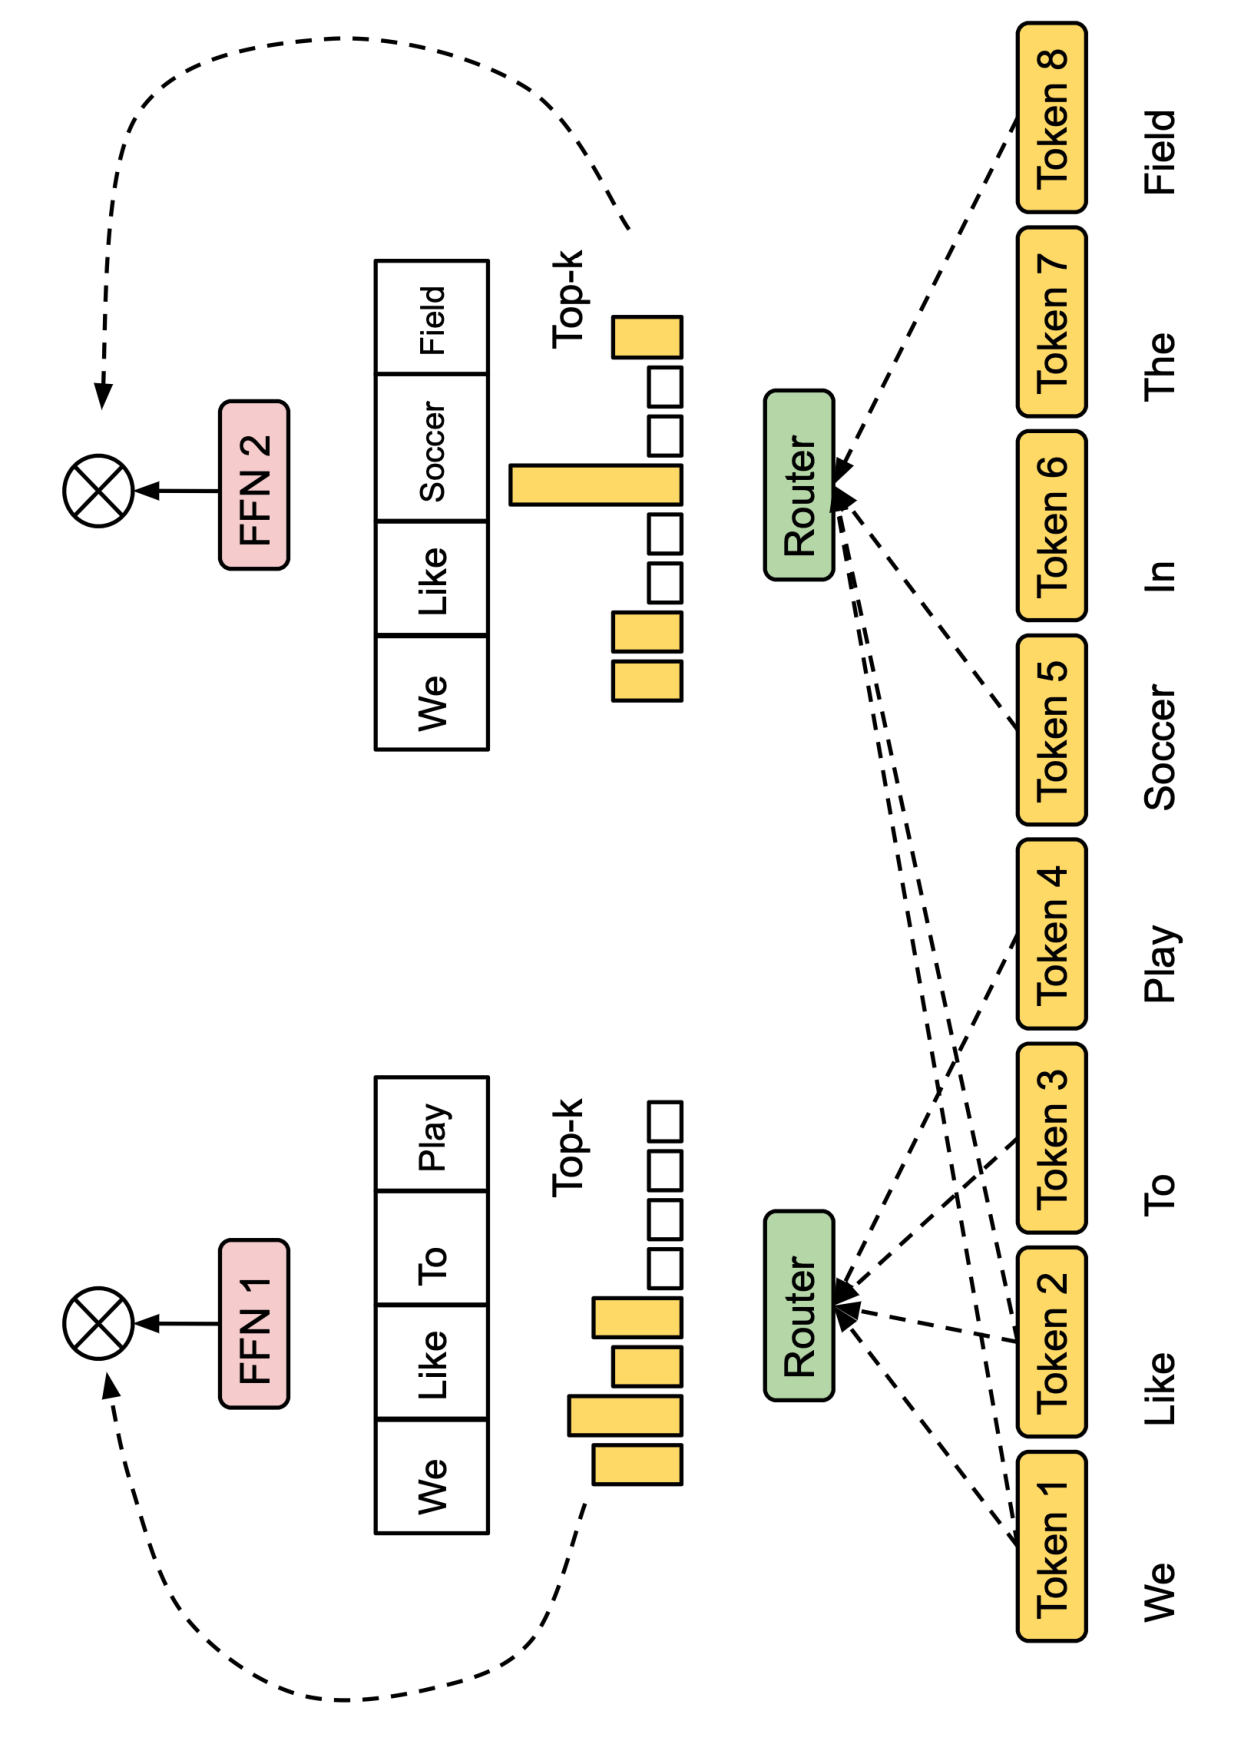
\includegraphics[angle=-90,width=0.9\linewidth]{figures/expert-to-token.pdf}
    \caption{“专家选择词元”的策略\cite{Zhou2022MixtureofExpertsWE}}
    \label{fig:expert-to-tokem}
\end{figure}


具体的路由过程如下：
\begin{enumerate}
    \item \textbf{计算亲和度分数：} 与经典路由类似，首先计算每个词元与每个专家之间的亲和度分数。对于输入词元表征矩阵$X \in \mathbb{R}^{n \times d}$和专家嵌入矩阵$W_g \in \mathbb{R}^{d \times E}$，亲和度分数矩阵$S \in \mathbb{R}^{n \times E}$通过softmax函数计算得出：
    \begin{equation}
        S = \text{softmax}(X \cdot W_g)
    \end{equation}
    \item \textbf{专家选择词元：} 对分数矩阵$S$的转置$S^T$进行操作，每个专家（$S^T$的每一行）从中选择分数最高的$k$个词元。这一步确定了每个专家处理的词元集合。
    \item \textbf{计算与输出：} 被选中的词元被送入对应的专家网络进行计算。由于一个词元可能被多个专家选中，它会从多个专家那里获得输出。最终的输出是所有处理过该词元的专家输出的加权和。
\end{enumerate}
通过这种方式，每个专家的计算负载是完全相同的（都处理$k$个词元），从而无需额外的负载均衡损失。同时，一个词元被处理的次数（即激活的专家数）是可变的，这取决于它被多少专家选为“Top-k”亲和度的词元，从而实现了对不同词元的计算资源的动态分配。但是，由于分配时需要知道整句句子的信息，这类方法对编码器模型较为友好，对解码器模型应用起来则较为困难。


\subsection{基于输入难度的动态路由}
与专家选择路由不同，另一类方法保留了“词元选择专家”的框架，但将激活的专家数量$k$从一个固定的超参数变为一个根据输入动态决定的变量。其核心假设是“更难的任务需要更多的专家”。Huang等人提出的动态路由机制\cite{Huang2024HarderTN}（图\ref{fig:top-p-routing}）是其中的一个代表。

\begin{figure}[h]
    \centering
    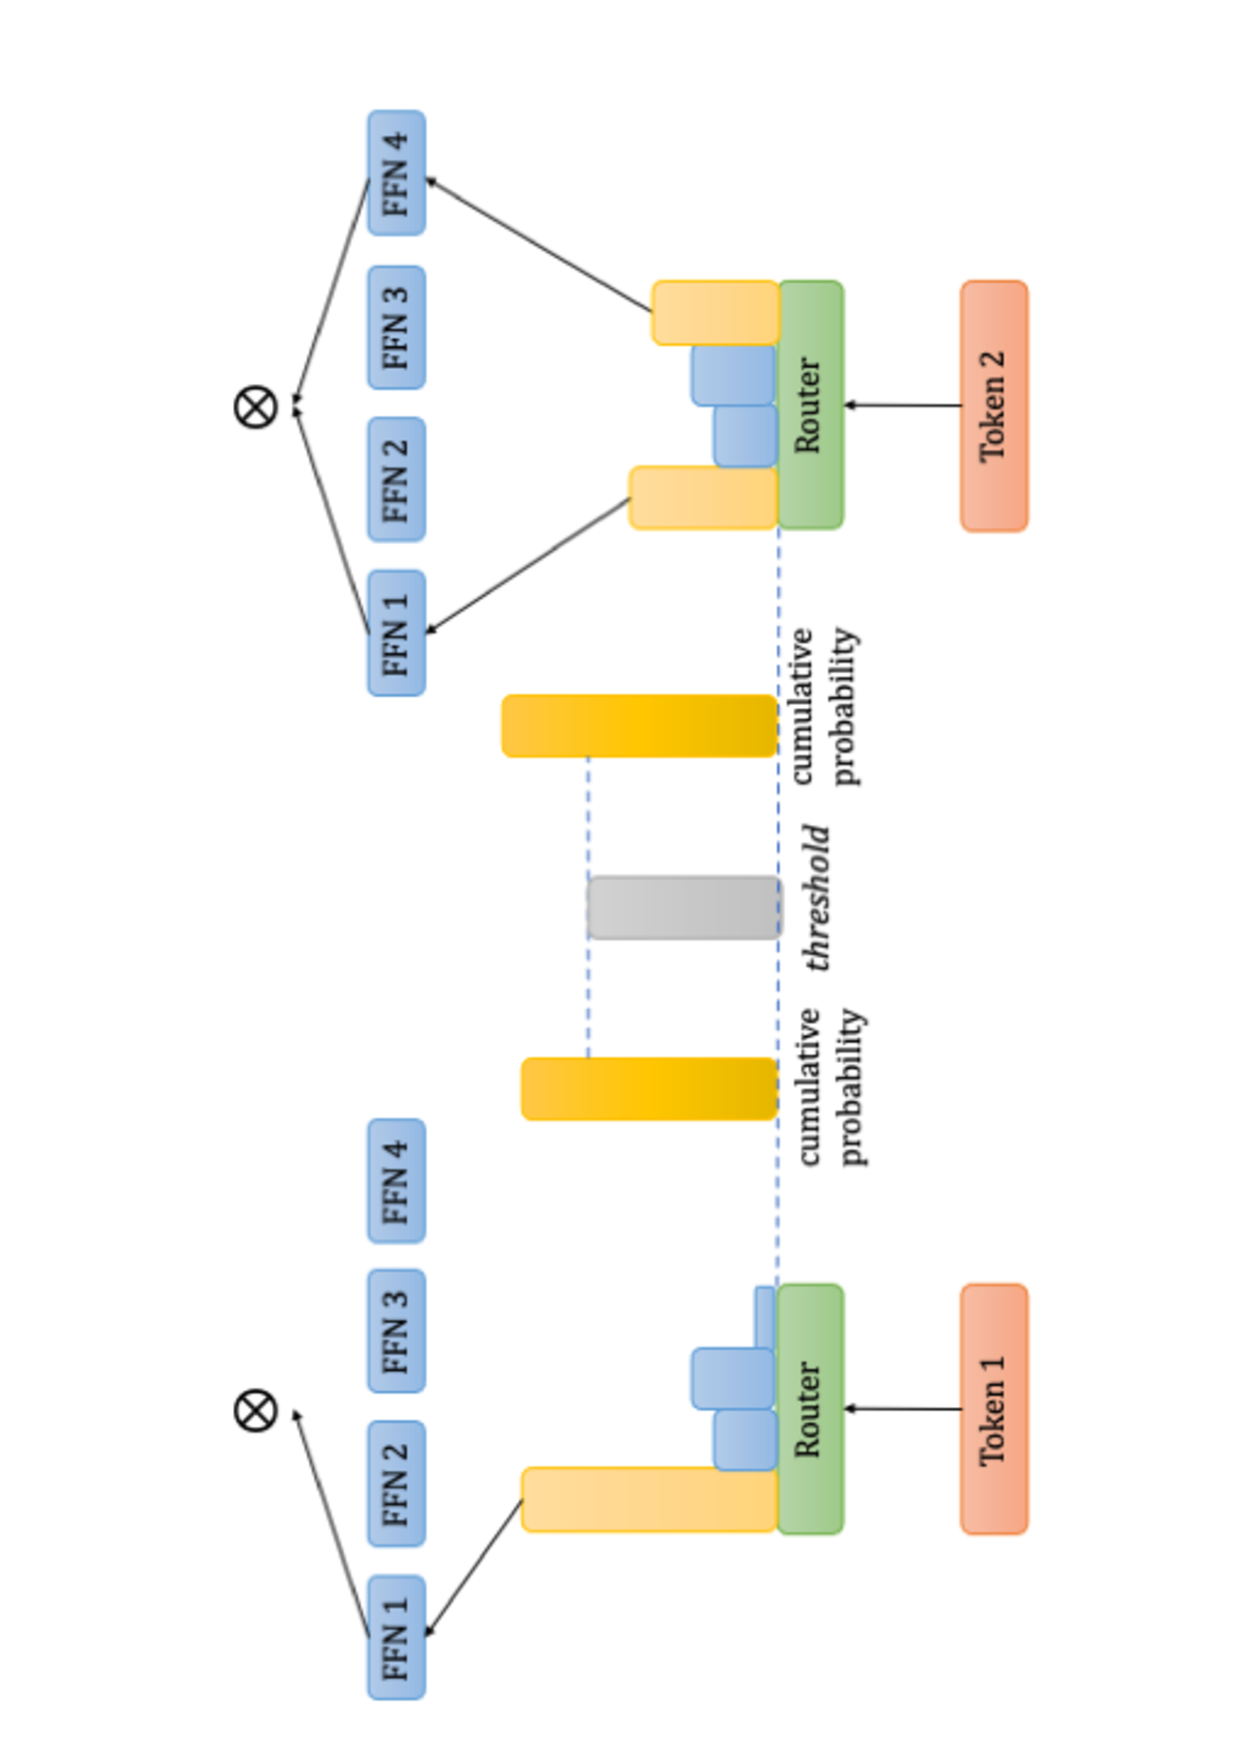
\includegraphics[angle=-90,width=0.9\linewidth]{figures/top-p-routing.pdf}
    \caption{基于置信度的专家选择策略\cite{Huang2024HarderTN}}
    \label{fig:top-p-routing}
\end{figure}

该方法引入了一种基于置信度的专家选择策略，其工作流程如下：
\begin{enumerate}
    \item \textbf{计算专家概率：} 对于一个输入词元，路由器首先计算出一个概率分布$P$，表示该词元分配给各个专家的概率。
    \item \textbf{动态专家选择：} 将专家按照概率从高到低排序。然后，模型会累加这些概率，直到累积概率超过一个预设的阈值$p$（例如0.9）。被累加的这些专家就是最终被激活的专家。激活的专家数量$t$由下式决定：
    \begin{equation}
        t = \arg\min_k \left( \sum_{i=1}^{k} P_i \geq p \right)
    \end{equation}
    其中$P_i$是排序后第$i$个专家的概率。这种策略也被称为Top-P路由。
    \item \textbf{动态损失函数：} 为了防止模型通过降低所有专家的概率来“作弊”并激活大量专家，该方法引入了一个动态损失函数$L_d$来鼓励路由器产生更稀疏（即更集中）的概率分布。这个损失函数实际上是概率分布$P$的熵：
    \begin{equation}
        L_d = \sum_{i=1}^{E} -P_i \log(P_i)
    \end{equation}
    通过最小化这个熵损失，模型被激励将概率集中在少数几个专家上，从而在没有明确限制的情况下也能实现稀疏激活。
\end{enumerate}
这种机制使得模型能够为它认为“简单”的词元（即路由器给出一两个高置信度专家）分配较少的专家，而为“复杂”的词元（即路由器给出的专家概率分布较为平坦）分配更多的专家，实现了更精细化的计算资源分配。

\subsection{动态混合专家模型 (DynMoE)}
Guo等人提出的动态混合专家模型（Dynamic Mixture of Experts, DynMoE）\cite{Guo2024DynamicMO}则是一种更为彻底的自适应方法，它不仅能自动决定每个词元激活的专家数量，还能在训练过程中动态地调整专家总数（图\ref{fig:dynmoe}）。

\begin{figure}[h]
    \centering
    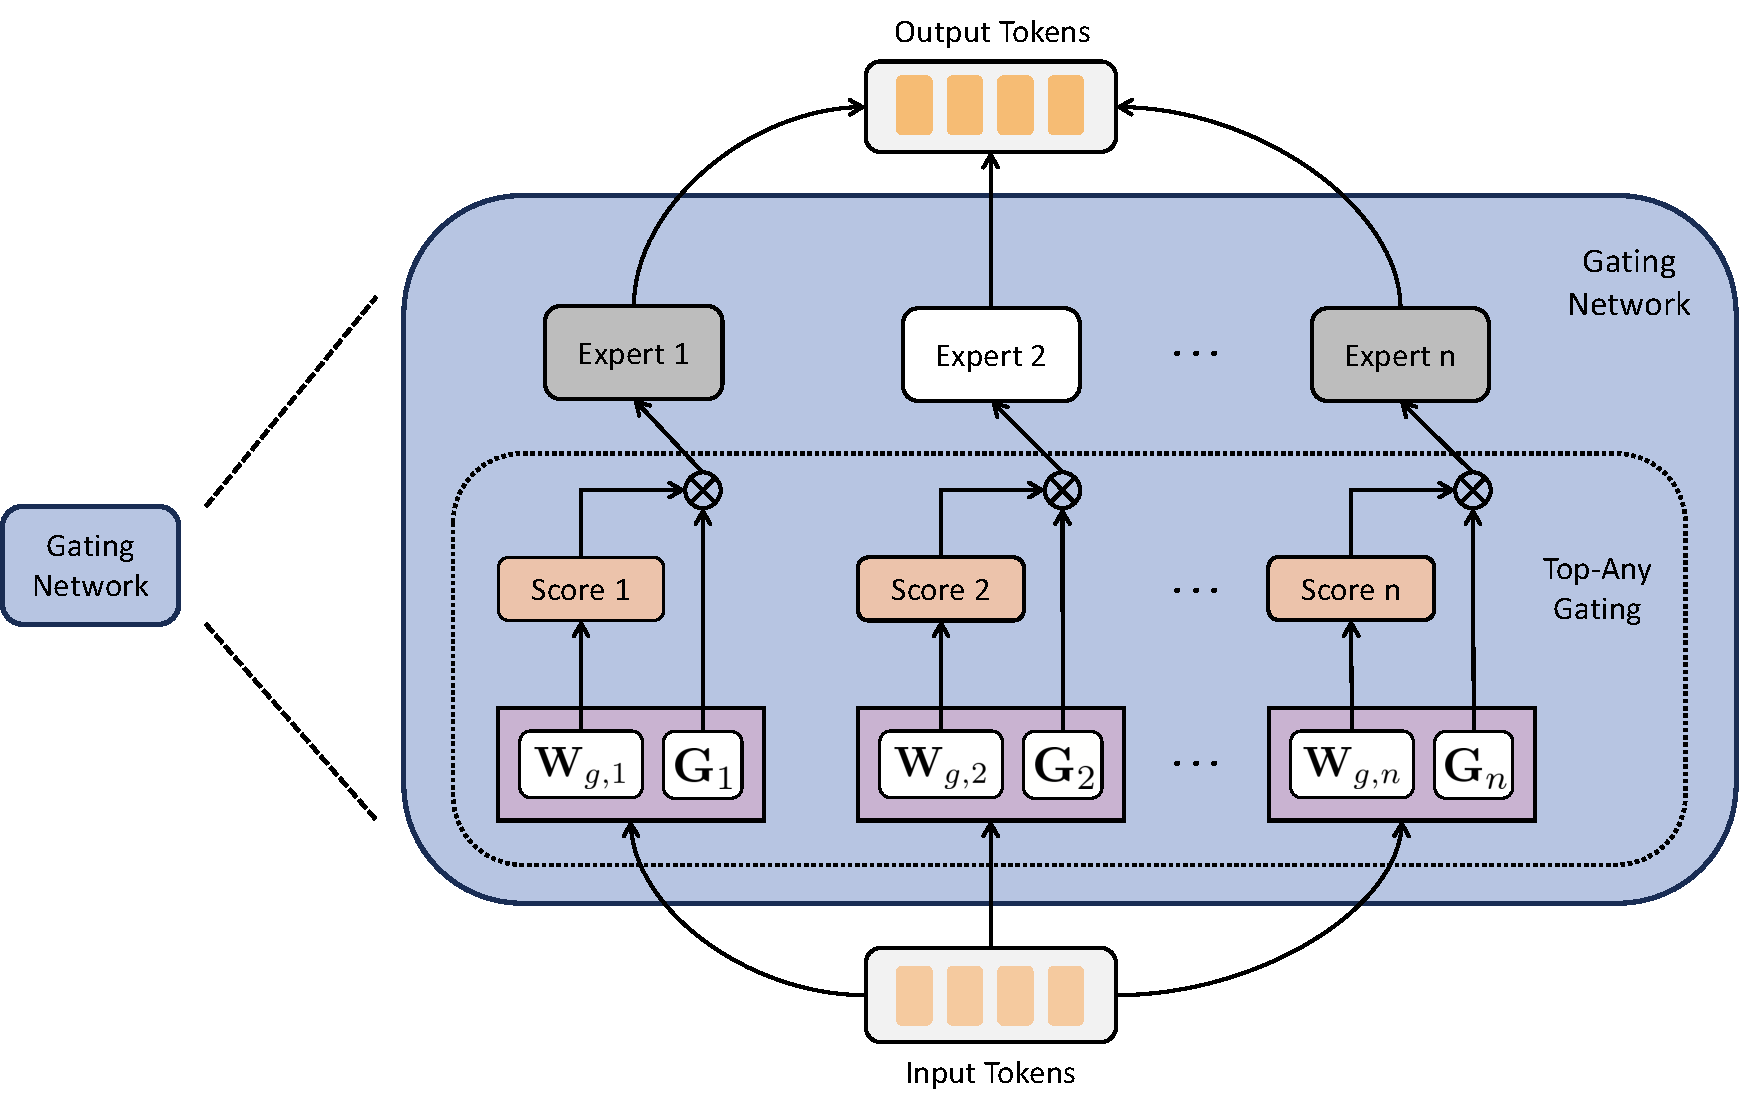
\includegraphics[width=0.85\linewidth]{figures/dynmoe.pdf}
    \caption{DynMoE架构\cite{Guo2024DynamicMO}}
    \label{fig:dynmoe}
\end{figure}

DynMoE的核心创新包括：
\begin{enumerate}
    \item \textbf{Top-any门控机制：} 该机制将专家选择问题建模为一个多标签分类问题。每个专家都被视为一个独立的类别。对于输入词元$x$和专家嵌入$W_g$，模型首先计算它们之间的余弦相似度分数$s(x)$。然后，每个专家$e$都有一个可学习的激活阈值$G_e$。如果词元$x$与专家$e$的相似度分数经过sigmoid函数变换后大于该专家的阈值，则该专家被激活：
    \begin{equation}
        g(x)_e = 
        \begin{cases}
            1 & \text{if } \sigma(s(x)_e) > \sigma(G_e) \\
            0 & \text{otherwise}
        \end{cases}
    \end{equation}
    这种机制允许一个词元激活任意数量的专家，包括零个。为了防止在推理过程中丢弃词元，对于没有激活任何专家的词元，系统会退回到Top-1路由策略。

    \item \textbf{专家数量自适应调整：} 在训练过程中，DynMoE会监控专家的使用情况，并动态地增加或删减专家。
    \begin{itemize}
        \item \textbf{增加专家：} 如果在一个训练批次中，存在一些词元没有激活任何专家，模型会根据这些词元的平均嵌入向量来初始化一个新的专家。
        \item \textbf{移除专家：} 如果一个专家在连续的很多训练步骤中都未被任何词元激活，它就会被视作冗余专家并被移除。
    \end{itemize}
    \item \textbf{新的辅助损失函数：} 为了在这种灵活的路由机制下保证稀疏性，DynMoE引入了一个“稀疏且简单的门控损失”（sparse and simple gating loss）。该损失由两部分组成：
    \begin{itemize}
        \item \textbf{多样性损失（Diversity Loss）：} $L_{div} = ||W_g^T W_g - I||_F^2$。该损失鼓励不同专家的嵌入向量相互正交，从而使它们学习到更多样化的特征。
        \item \textbf{简洁性损失（Simplicity Loss）：} $L_{sim} = \sum_e ||w_{g,e}||_2$。该损失对专家嵌入向量的L2范数进行惩罚，以维持数值稳定性。
    \end{itemize}
\end{enumerate}
DynMoE通过上述机制，实现了对MoE模型超参数（激活专家数$k$和专家总数$E$）的自动调整，极大地减少了模型设计和调优所需的人工和计算成本。

\section{前馈网络之外的混合专家模型}
\label{sec:moe_beyond_ffn}
经典的混合专家模型主要将专家网络应用于Transformer中的前馈网络 (FFN) 部分。然而，条件计算 (Conditional Computation) 的思想具有更广泛的适用性。学术界已经开始探索将混合专家机制与其他模块相结合，甚至重塑整个模型架构的计算流程，旨在将模型的动态性和稀疏性提升到新的水平。本节将介绍若干代表性的前沿工作，它们将混合专家模型的思想从前馈网络扩展到了注意力机制、整体模块组合乃至记忆等多个维度。

\subsection{混合注意力头（MoA）}
混合注意力头 (Mixture of Attention Heads, MoA) \cite{Zhang2022MixtureOA} 将混合专家模型的理念直接应用于多头注意力机制 (Multi-Head Attention, MHA) 中，而非传统的前馈网络层（图\ref{fig:moa}）。其核心思想是，并非每个输入词元都需要所有注意力头的参与，而是可以根据上下文动态地选择一个最相关的子集。

\begin{figure}[h]
    \centering
    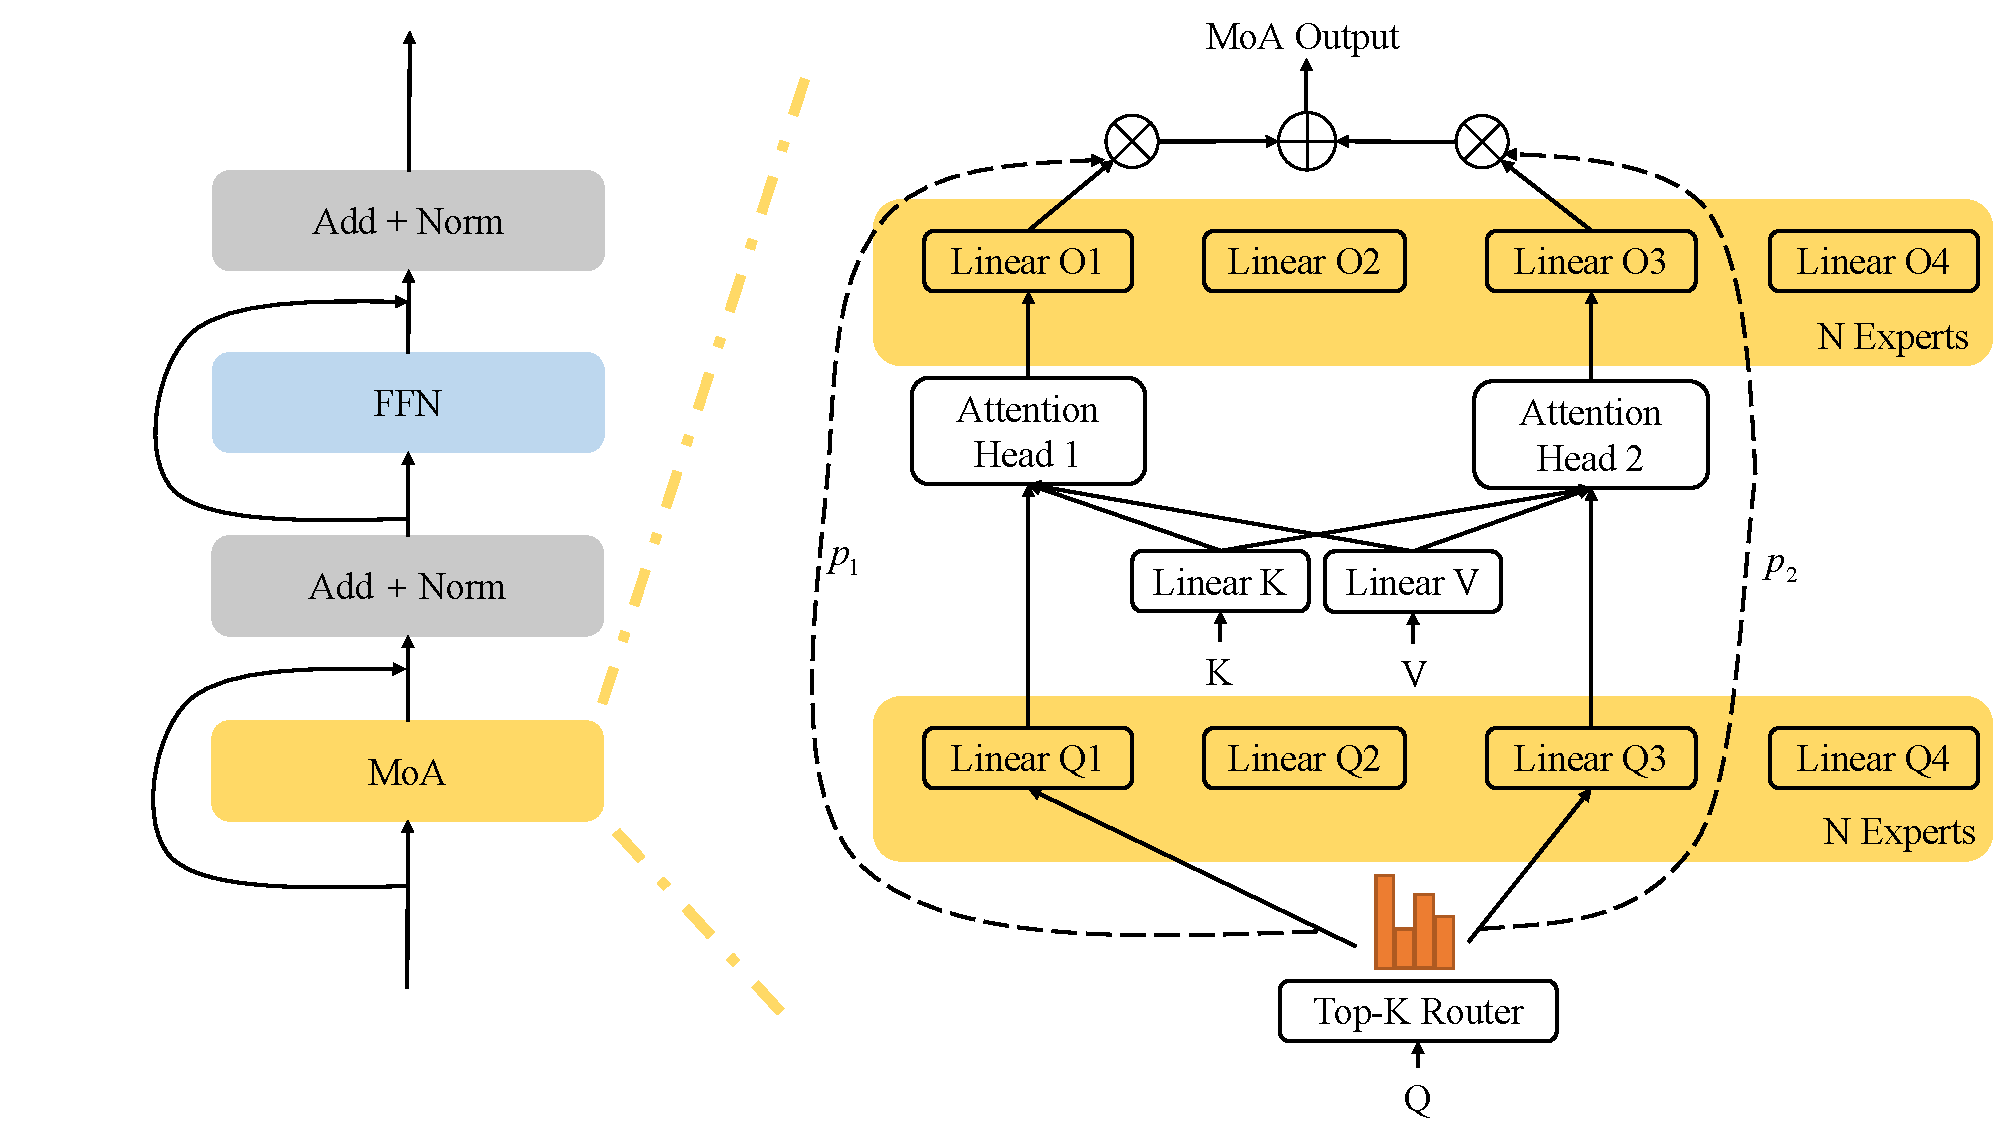
\includegraphics[width=0.9\linewidth]{figures/MoA.pdf}
    \caption{混合注意力头架构\cite{Zhang2022MixtureOA}}
    \label{fig:moa}
\end{figure}

在MoA架构中，存在一个包含$N$个“注意力专家” (Attention Experts) 的专家池，其中每个专家本质上就是一个拥有独立参数的注意力头。对于输入序列中的每一个词元$x$，一个可学习的路由器 (Router) 会计算该词元与所有$N$个注意力专家的亲和度得分，并从中选择得分最高的$k$个专家来处理该词元。最终的注意力输出是这$k$个被激活专家输出的加权和，其权重由路由器的得分归一化后得到。

为了在扩大专家数量的同时控制计算和参数开销，MoA采用了一种高效的设计: 它在所有注意力专家之间共享键 (Key, $W^K$) 和值 (Value, $W^V$) 的投影矩阵，仅保留查询 (Query, $W^Q$) 和输出 (Output, $W^O$) 的投影矩阵为每个专家私有。这样，计算代价高昂的$K, V$矩阵变换只需执行一次，而每个专家只需进行轻量级的$Q$向量投影和输出计算。

与标准混合专家模型类似，MoA也引入了辅助损失函数$L_{\text{aux}}$来促进专家间的负载均衡，防止少数专家被过度使用。其形式如下:
\begin{equation}
    L_{\text{aux}}(Q) = N \cdot \sum_{i=1}^{N} f_i \cdot P_i
\end{equation}
其中，$Q$代表一个批次中的所有词元查询，$N$是专家总数，$f_i$是第$i$个专家被分配到的词元数量占比，$P_i$是第$i$个专家在整个批次中获得的路由门控概率之和。该损失函数旨在平衡每个专家的使用频率和门控权重，鼓励模型更均匀地利用所有专家。实验证明，MoA能够在提升模型性能的同时，保持计算效率，并为模型可解释性提供了新的视角，因为不同的注意力专家倾向于学习不同的语言功能\cite{Zhang2022MixtureOA}。

\subsection{混合深度（MoD）}
混合深度 (Mixture-of-Depths, MoD)\cite{Raposo2024MixtureofDepthsDA} 是一种旨在动态分配计算资源的架构，它允许不同的词元在模型中经历不同数量的计算层，即拥有不同的计算“深度”。与传统的混合专家模型在宽度上扩展 (选择不同的专家) 不同，MoD在深度上进行稀疏化 (选择是否执行计算)（图\ref{fig:mod}）。

\begin{figure}[h]
    \centering
    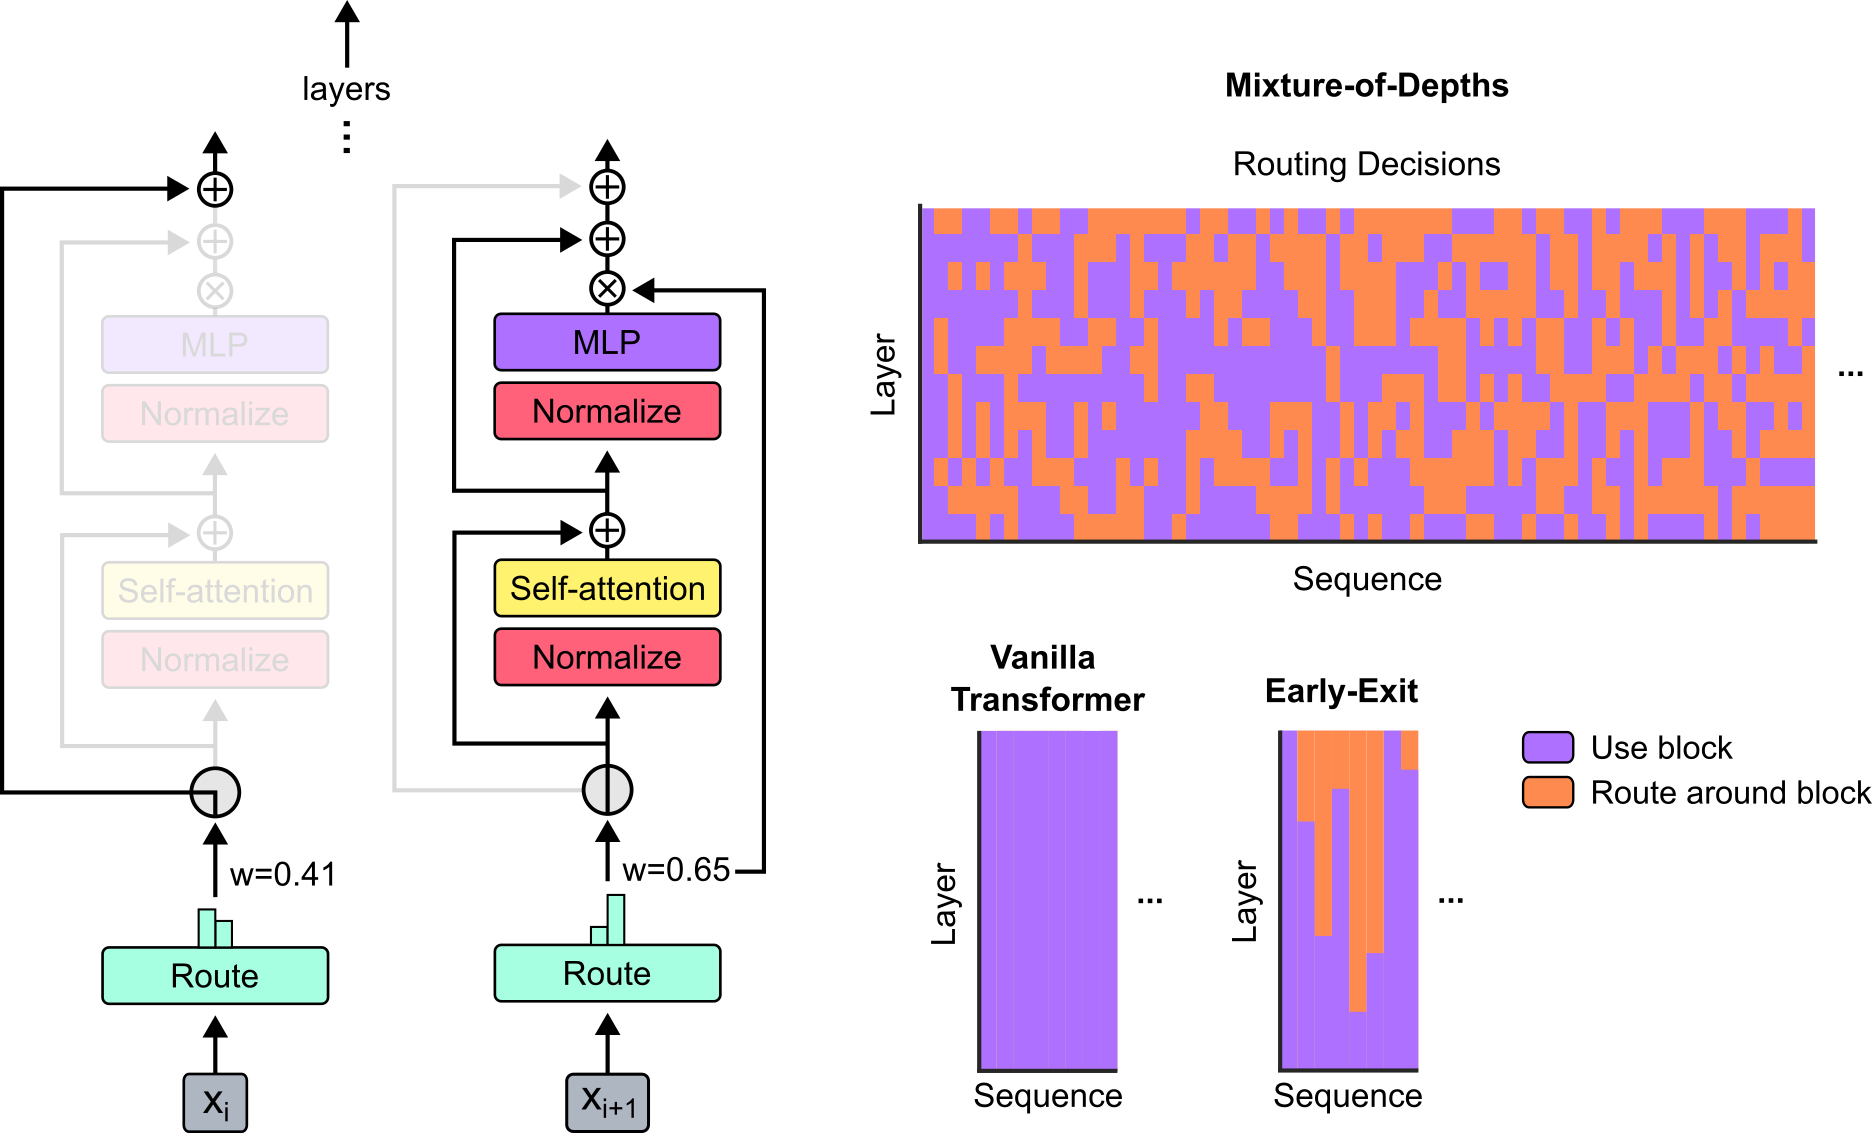
\includegraphics[width=1.0\linewidth]{figures/mod.png}
    \caption{混合深度架构\cite{Raposo2024MixtureofDepthsDA}}
    \label{fig:mod}
\end{figure}

其核心机制是，在Transformer的每个块 (Block) 前都设置一个路由器。对于输入序列中的每个词元，路由器会决定该词元是进入该块进行标准的自注意力和前馈网络计算，还是直接通过残差连接“跳过”该块。为了维持固定的计算预算并与现代硬件兼容，MoD采用了“专家选择” (Expert Choice)\cite{Zhou2022MixtureofExpertsWE} 的路由策略。在此策略中，并非由词元选择路径，而是由每个计算块 (被视为“专家”) 从所有输入词元中选择亲和度最高的$k$个词元进行处理。其余的$S-k$个词元则被跳过。

这种方式确保了每个块处理的词元数量是恒定的$k$，从而使计算图保持静态，极大地提升了训练和推理的效率。模型的计算开销仅与容量因子$k/S$成正比，而与序列长度无关。一个词元的最终计算路径由其在各层被路由决策的序列决定，例如一个词元可能跳过浅层块，但在深层块中被处理。

由于“专家选择”在训练时需要获取整个序列的信息来确定top-k，这在自回归生成任务的推理阶段是不可行的 (因为未来的词元尚不存在)。为了解决这个问题，MoD提出训练一个辅助的预测性路由器 (predictive router)，该路由器仅基于当前词元的信息来预测其是否会被主路由器选中，从而在推理时实现因果一致的动态路由\cite{Raposo2024MixtureofDepthsDA}。

\subsection{混合模块（MoM）}
混合模块（Mixture-of-Modules, MoM）\cite{Gong2024MixtureofModulesRT} 是一种颠覆性的架构，它彻底打破了传统Transformer模型固定的、自下而上的分层计算模式。其核心思想是将整个Transformer重塑为一个由基础模块 (Modules) 构成的集合，并通过动态路由来为每个词元“组装”出一个独特的计算图（图\ref{fig:mixtureofmodules}）。

\begin{figure}[h]
    \centering
    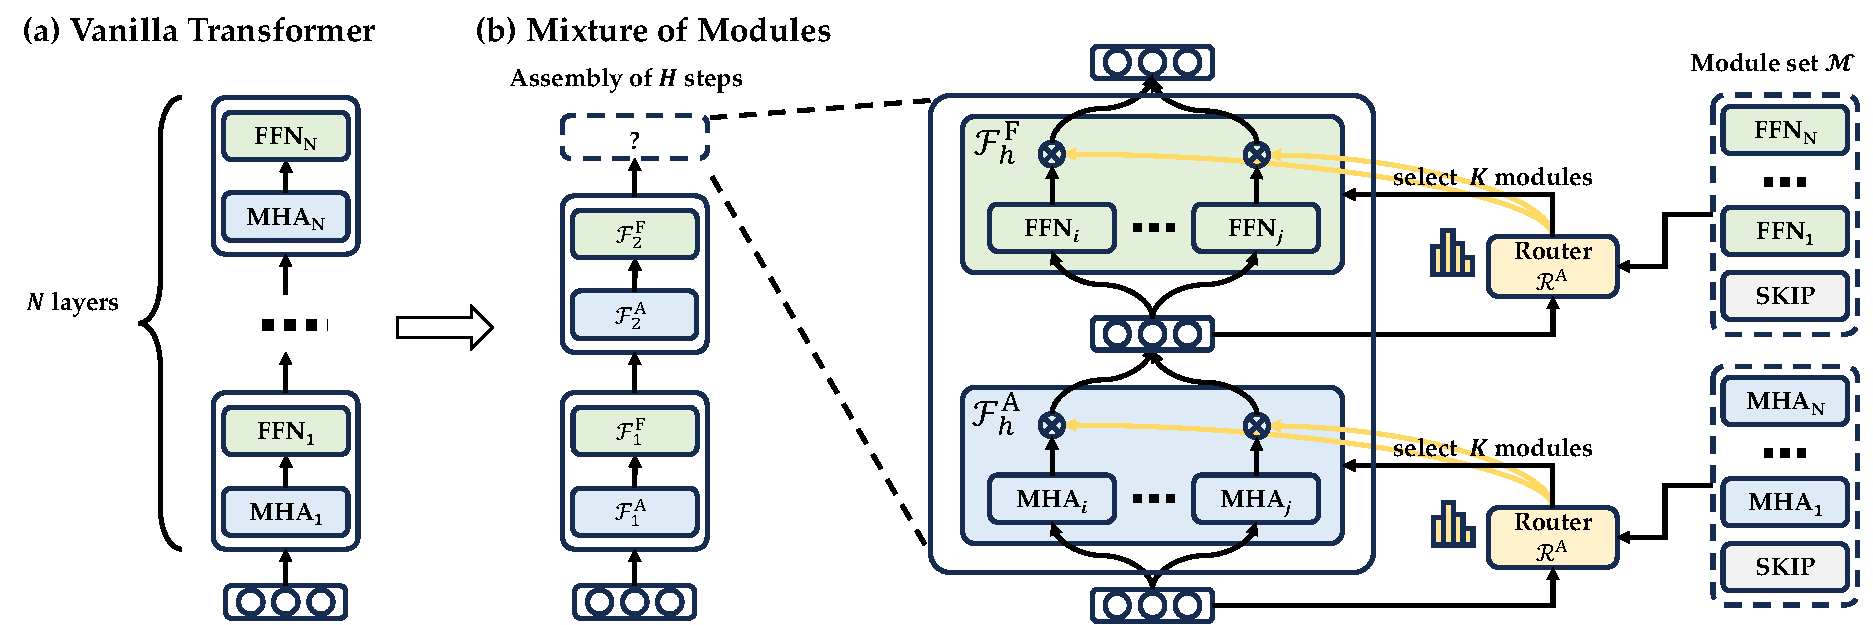
\includegraphics[width=1.0\linewidth]{figures/mixtureofmodules.pdf}
    \caption{混合模块架构\cite{Gong2024MixtureofModulesRT}}
    \label{fig:mixtureofmodules}
\end{figure}

MoM架构包含一个由多个独立的多头注意力机制模块和前馈网络模块组成的“模块池”。在处理每个词元时，计算过程不再是依次通过固定的第1层、第2层……，而是分为多个迭代步骤。在每个步骤中，模型通过两个独立的路由器——一个用于多头注意力机制模块，另一个用于前馈网络模块——从模块池中各自选择$K$个最合适的模块。这些被选中的模块的输出通过路由权重进行加权求和，形成该步骤的最终输出，并作为下一步的输入。整个前向传播过程就是这样一个动态构建和执行计算路径的过程。

与依赖于前一层输出的传统模型不同，MoM的路由器在做决策时需要感知历史选择信息。为此，MoM的路由器内部集成了一个门控循环单元（Gated Recurrent Unit, GRU）\cite{Cho2014LearningPR}，其隐藏状态$s_h^X$在每个组装步骤$h$中进行更新:
\begin{equation}
    s_h^X = \text{GRU}^X(x_h, s_{h-1}^X), \quad X \in \{\text{MHA}, \text{FFN}\}
\end{equation}
其中$x_h$是当前步骤的输入，$s_{h-1}^X$是上一状态。路由权重$r_h^X$则由当前状态$s_h^X$通过一个线性变换得到:
\begin{equation}
    r_h^X = W^X s_h^X
\end{equation}
这种设计允许路由决策具有记忆性，从而能够构建出更加复杂和协调的计算路径。

MoM不仅为Transformer的过参数化问题提供了新的解决方案，还统一了层跳过 (Layer-skipping)\cite{Teerapittayanon2016BranchyNetFI,Xin2021BERxiTEE,Elhoushi2024LayerSkipEE}、参数共享\cite{Dehghani2018UniversalT,Lan2019ALBERTAL}和混合专家等多种动态计算机制的框架\cite{Gong2024MixtureofModulesRT}。

\subsection{混合递归 (MoR)}
混合递归（Mixture-of-Recursions, MoR）\cite{Bae2025MixtureofRecursionsLD} 是一个统一了参数共享和自适应计算两大效率提升范式的框架（图\ref{fig:mor_overview}）。它基于循环Transformer（Recursive Transformer）\cite{Bae2024RelaxedRT,Fan2024LoopedTF,Giannou2023LoopedTA,Yang2023LoopedTA,Saunshi2025ReasoningWL} 的思想，即在多个计算步骤中重复使用同一组共享的层（一个“递归块”），但其创新之处在于，每个词元所经历的递归“深度” （即重复次数） 是动态可学习的。

\begin{figure}[h]
    \vspace{-7pt}
    \centering
    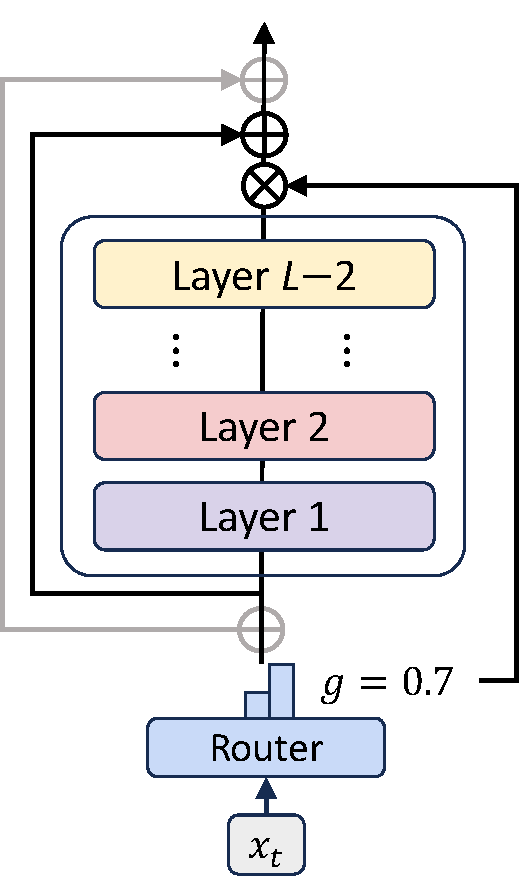
\includegraphics[width=0.23\columnwidth]{figures/overview/overview_main1.pdf}
    \hspace{23pt}
    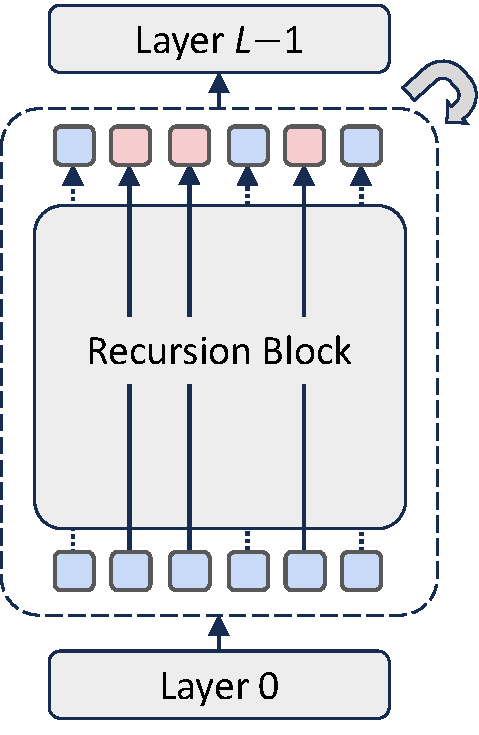
\includegraphics[width=0.238\columnwidth]{figures/overview/overview_main2.pdf}
    \hspace{7pt}
    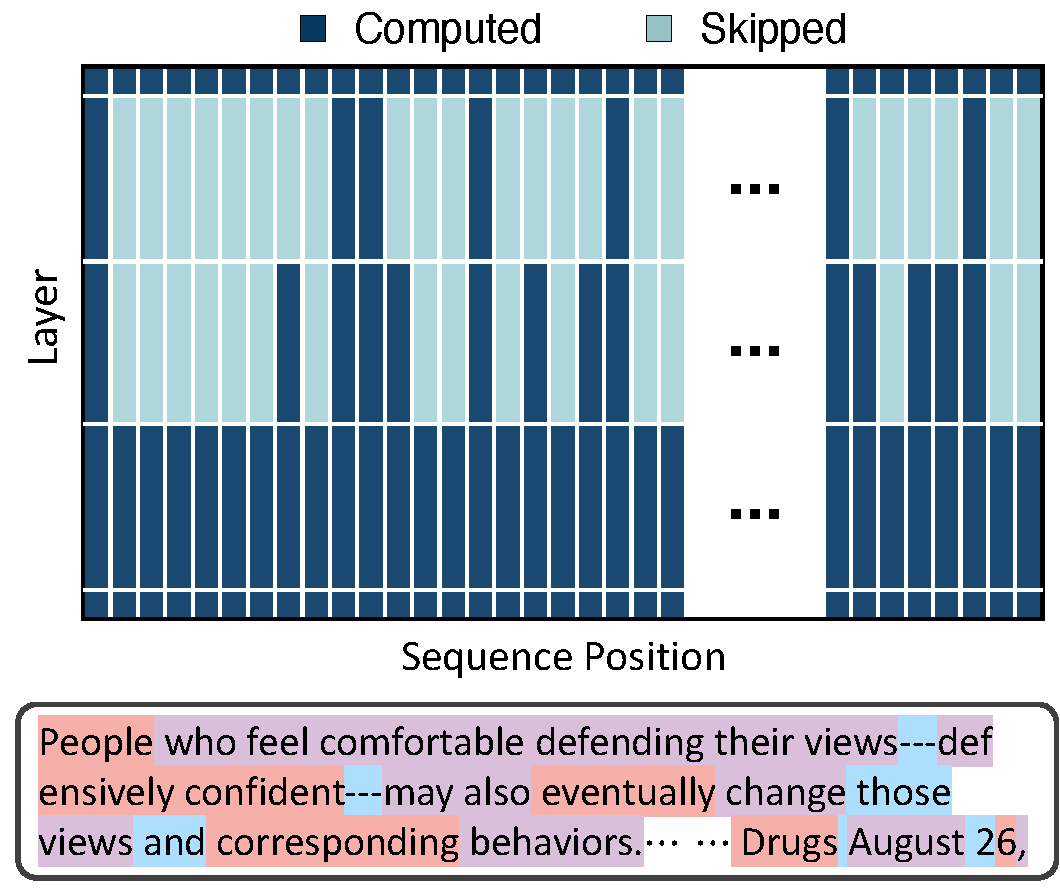
\includegraphics[width=0.42\columnwidth]{figures/overview/overview_main3.pdf}
    \caption{MOR的示意图\cite{Bae2025MixtureofRecursionsLD}}
    \label{fig:mor_overview}
\end{figure}

MoR的核心是一个轻量级路由器，它为输入序列中的每个词元$x_t$分配一个特定的递归次数$N_t$。这意味着，模型可以为它认为“困难”的词元分配更多的计算步骤（更大的$N_t$），而为“简单”的词元分配更少的计算步骤，从而实现细粒度的、自适应的计算资源分配。这种机制被类比为模型的“思考深度”。

该架构不仅通过参数共享大幅减少了模型的参数量，还通过动态路由显著降低了前向传播所需的总计算量 (FLOPs)。此外，MoR为动态深度模型设计了专门的键值缓存（KV Caching）策略:
\begin{itemize}
    \item \textbf{递归维度缓存（Recursion-wise Caching）}: 每个递归深度层级都拥有自己独立的KV缓存。只有在特定深度被激活的词元，其键值对才会被缓存并用于该层的注意力计算。
    \item \textbf{递归KV共享（Recursive KV Sharing）}: 所有词元在第一个递归步骤中产生的键值对被缓存，并在后续所有递归步骤中共享使用。
\end{itemize}
这些策略进一步优化了推理过程中的内存占用和访存效率。实验表明，MoR在同等训练FLOPs和更小模型尺寸下，能够达到乃至超越标准Transformer和固定深度循环模型的性能，形成了一个新的帕累托前沿\cite{Bae2025MixtureofRecursionsLD}。

\subsection{混合记忆（Mixture-of-Memories）}
混合记忆（Mixture-of-Memories, MoM）（图\ref{fig:mixtureofmemories}）\cite{Du2025MoMLS} 将混合专家的思想应用于线性序列模型（如线性注意力、状态空间模型等）的核心瓶颈——其固定大小的记忆状态（memory state）。传统线性模型将整个历史信息压缩到一个单一的记忆状态中，容易导致“记忆干扰”（memory interference）和容量受限，在需要精确回忆长距离信息的任务上表现不佳。

\begin{figure}[h]
    \centering
    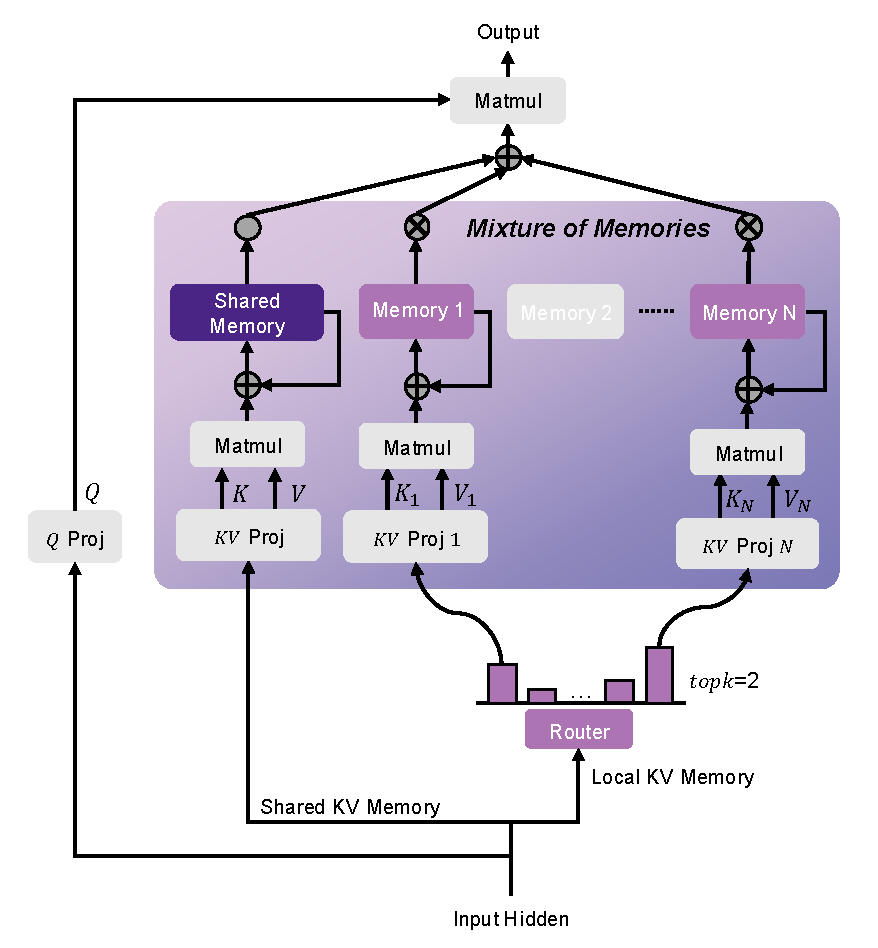
\includegraphics[width=0.8\linewidth]{figures/mom_fig1.pdf}
    \caption{混合记忆架构\cite{Du2025MoMLS}}
    \label{fig:mixtureofmemories}
\end{figure}

MoM架构的创新之处在于引入了多个独立的记忆状态，称之为“记忆专家”（Memory Experts）。其工作流程如下:
\begin{enumerate}
    \item \textbf{路由}: 对于每个输入词元$x_t$，一个路由器会计算其与所有$M$个记忆专家的相关性得分，并选择top-k个最相关的记忆进行更新。
    \item \textbf{并行更新}: 输入词元$x_t$被投影为$k$组独立的键值对 $(k_t^m, v_t^m)$，分别用于更新被选中的$k$个记忆状态$M_{t-1}^m$:
    \begin{equation}
        M_t^m = M_{t-1}^m + (k_t^m)^T v_t^m
    \end{equation}
    而未被选中的记忆状态则保持不变，$M_t^j = M_{t-1}^j$，从而避免了不相关信息的干扰。
    \item \textbf{记忆混合与查询}: 所有被激活的记忆状态根据路由器的门控权重$g_t^{(m)}$加权求和，形成一个临时的“混合记忆”$\bar{M_t}$:
    \begin{equation}
        \bar{M_t} = \sum_{m \in \text{TopK}(x_t)} g_t^{(m)} M_t^m
    \end{equation}
    最终的输出$o_t$由查询向量$q_t$与该混合记忆相互作用产生: $o_t = q_t \bar{M_t}$。
\end{enumerate}
通过将信息分流到不同的记忆通道，混合记忆极大地增强了模型的总记忆容量，并显著减轻了记忆干扰问题。这使得它在保持线性复杂度的同时，在各种依赖长程记忆的任务上性能大幅超越了其他线性模型，甚至能与标准的Transformer模型相媲美\cite{Du2025MoMLS}。

\section{专家选择的软性化}
经典的混合专家模型依赖于离散的路由决策，即为每个词元（token）选择或“硬性”分配特定的专家。这种离散性虽然实现了计算的稀疏化，但也使得路由器的训练变得困难，因为它本身不可微，必须依赖梯度直通估计（STE）等近似方法，这可能导致训练不稳定或收敛到次优解。为了解决这一问题，研究者们探索了将路由机制“软性化”的思路，通过引入可微的操作来替代离散的专家选择，从而实现端到端的稳定训练。

\subsection{Soft MoE}
Puigcerver等人提出的Soft MoE\cite{Puigcerver2023FromST} 是一种完全可微的稀疏Transformer变体。它与传统混合专家模型的核心区别在于，它执行的是隐式的“软性”分配，而非显式的“硬性”分配（图\ref{fig:SoftMoE}）。

\begin{figure}[h]
    \centering
    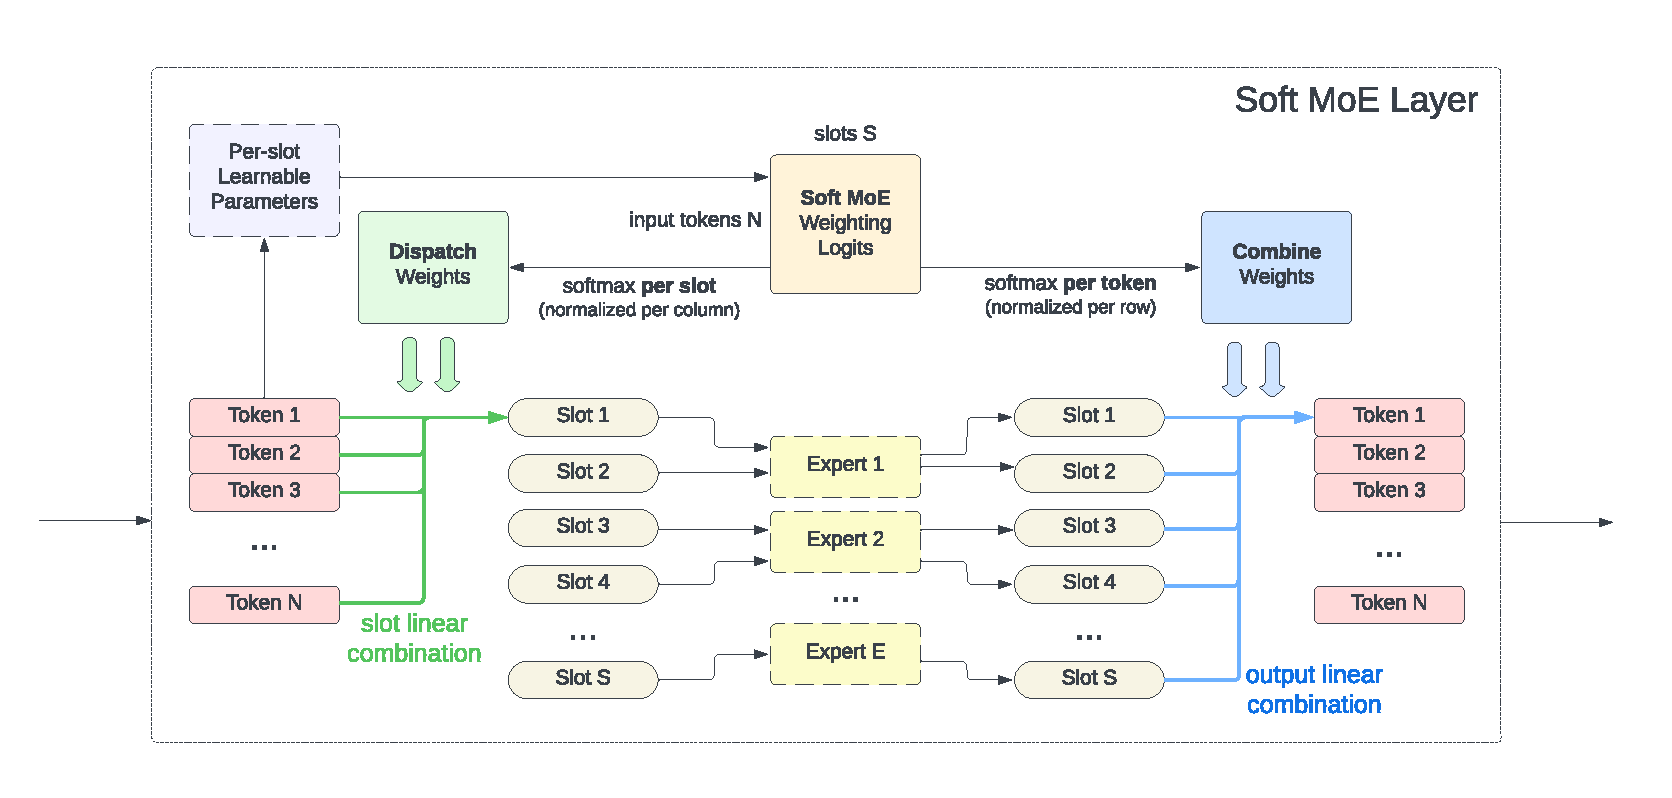
\includegraphics[width=1.0\linewidth]{figures/SoftMoE_diagram.pdf}
    \caption{Soft MoE的路由细节\cite{Puigcerver2023FromST}}
    \label{fig:SoftMoE}
\end{figure}

在经典的“词元选择专家”模式中，一个词元会被路由到少数几个专家。而在Soft MoE中，每个专家的输入不再是某个特定的词元，而是所有输入词元的加权平均。具体来说，假设一个序列的输入为 $X \in \mathbb{R}^{T \times d}$（$T$为序列长度，$d$为词元表征维度），专家数量为$N$，每个专家处理$p$个“槽位”（slot）。Soft MoE会为每个槽位（共$N \times p$个）生成一个输入表征$\tilde{x}$，该表征是所有$T$个输入词元的加权和。其槽位输入矩阵$\tilde{X} \in \mathbb{R}^{(N \cdot p) \times d}$ 的计算方式如下：
\begin{equation}
    \tilde{X} = D^T X
\end{equation}
其中，$D \in \mathbb{R}^{T \times (N \cdot p)}$ 是一个“分发权重”（Dispatch Weights）矩阵，通过对词元和槽位之间的亲和度得分进行softmax计算得到。这意味着每个槽位的输入都是对整个输入序列的一种“软性”关注。

在所有专家处理完各自的槽位输入后，模型的最终输出$Y$同样通过对所有专家槽位的输出$\tilde{Y}$进行加权求和得到：
\begin{equation}
    Y = C \tilde{Y}
\end{equation}
其中，$C \in \mathbb{R}^{T \times (N \cdot p)}$ 是“组合权重”（Combine Weights）矩阵，其计算方式与$D$类似。

通过这种方式，Soft MoE中的所有操作都是可微的，不再需要梯度估计。它避免了词元丢弃和负载不均衡问题，因为每个专家处理的计算量是固定的。实验表明，Soft MoE在保持混合专家模型优势的同时，训练过程更稳定，且性能优于传统的稀疏混合专家模型。

\subsection{SMEAR}
Muqeeth等人提出的SMEAR（Soft Merging of Experts with Adaptive Routing）\cite{Muqeeth2023SoftMO}提供了另一种实现路由软性化的思路。与Soft MoE混合（加权平均）词元输入不同，SMEAR的核心思想是混合专家的参数（图\ref{fig:smear}）。

\begin{figure}[h]
    \centering
    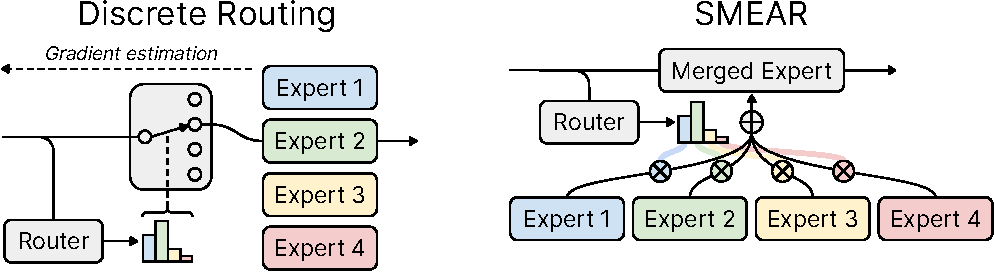
\includegraphics[width=1.0\linewidth]{figures/smear.pdf}
    \caption{SMEAR架构和普通混合专家模型的对比\cite{Muqeeth2023SoftMO}}
    \label{fig:smear}
\end{figure}

具体来说，对于一个输入$x$，路由器不再决定将$x$发送给哪个专家，而是计算出一组权重$G(x)$，用来对所有专家的参数进行加权平均，从而动态地构建出一个临时的“融合专家”（Merged Expert）。然后，输入$x$被这个融合专家处理，得到最终输出。其计算过程可以表示为：
\begin{equation}
    y = f(x, \theta_{\text{merged}}) \quad \text{其中} \quad \theta_{\text{merged}} = \sum_{i=1}^{N} G(x)_i \cdot \theta_i
\end{equation}
这里，$\theta_i$是第$i$个专家的参数，$G(x)_i$是路由器为当前输入$x$分配给第$i$个专家的权重，$\theta_{\text{merged}}$是融合后的专家参数，$f$代表专家网络（所有专家参数不同，但是专家网络对应的函数相同）。

SMEAR巧妙地将离散的路由选择问题转化为了连续的参数加权问题。由于整个计算过程完全可微，因此可以直接使用标准的反向传播算法进行端到端训练，无需任何梯度估计技巧。这种方法不仅避免了离散路由带来的训练不稳定性，还在经验上被证明优于使用梯度估计的路由方法以及基于元数据的启发式路由方法。定性分析也表明，通过SMEAR训练的专家网络表现出了显著的功能特化。

\section{极细粒度专家}
混合专家模型的另一个重要发展方向是追求“极细粒度”的专家设计。传统混合专家模型中的“专家”通常是完整的前馈神经网络（FFN）。而极细粒度专家则将“专家”的概念推向极致，将其简化为极小的计算单元，例如一个键值对（key-value pair）或者一个单神经元网络。这种设计使得模型可以在专家数量上扩展到前所未有的规模，同时保持计算量的可控性。

\subsection{乘积记忆存储器 (PKM)}
Lample等人提出的乘积记忆存储器（Product Key Memory, PKM）\cite{Lample2019LargeML}是极细粒度专家思想的早期探索。它将Transformer中的前馈网络层替换为一个大规模的、可学习的键值记忆（key-value memory）。这个记忆模块可以被视为一个拥有海量“专家”的混合专家模型层，其中每个“专家”就是一个简单的值向量（value）（图\ref{fig:PKM}）。

\begin{figure}[h]
    \centering
    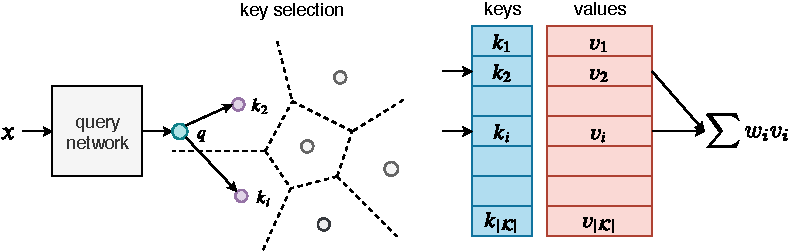
\includegraphics[width=1.0\linewidth]{figures/memory-crop.pdf}
    \caption{乘积记忆存储器的示意图\cite{Lample2019LargeML}}
    \label{fig:PKM}
\end{figure}

面对海量（例如百万级别）的密钥，穷举式的相似度计算是不可行的。为了高效地从中检索信息，PKM引入了“乘积量化”（Product Quantization）的思想来构建和查询密钥。具体来说，一个高维的密钥$k$被分解为两个低维子密钥$c_1$和$c_2$的拼接（concatenation），即$k = [c_1, c_2]$。整个密钥空间由两个较小的子密钥码本$C_1 \in \mathbb{R}^{N_s \times (d_k/2)}$和$C_2 \in \mathbb{R}^{N_s \times (d_k/2)}$的笛卡尔积隐式定义，其中$N_s = \sqrt{N}$是每个码本的大小，$d_k$是完整密钥的维度。这样，总的密钥数量可以达到$N = N_s^2$。

其选择过程分为两个阶段：
\begin{enumerate}
    \item \textbf{候选集生成}：对于一个输入$x$生成的查询向量$q$（同样被分解为$[q_1, q_2]$），模型首先在两个子码本中独立地进行快速的Top-$k_s$搜索，找出与$q_1$和$q_2$最相似的$k_s$个子密钥。
    \begin{gather}
        \mathcal{T}_1 = \text{TopK}_{k_s}(\{ q_1^T c_{1,i} \}_{i=1}^{N_s}) \\
        \mathcal{T}_2 = \text{TopK}_{k_s}(\{ q_2^T c_{2,j} \}_{j=1}^{N_s})
    \end{gather}
    其中$\mathcal{T}_1$和$\mathcal{T}_2$是选出的$k_s$个子密钥的索引集合。这两个集合中的子密钥组合起来，构成了一个包含$k_s^2$个完整密钥的候选集。理论上可以证明，与完整查询$q$最相似的Top-$k$密钥必定位于这个候选集中。
    \item \textbf{最终专家选择}：接下来，模型仅在这个小得多的候选集上计算完整的相似度得分，并从中选出最终的Top-$k$个密钥。对于候选集中的任意一个密钥$k_{ij} = [c_{1,i}, c_{2,j}]$（其中$i \in \mathcal{T}_1, j \in \mathcal{T}_2$），其与$q$的点积得分为$s_{ij} = q^T k_{ij} = q_1^T c_{1,i} + q_2^T c_{2,j}$。模型基于这$k_s^2$个得分选出最高的$k$个，其对应的索引集合记为$\mathcal{T}_{\text{final}}$。
\end{enumerate}

最终，模型的输出$y$是被选中的$k$个值向量$V_{ij}$的加权和，权重由这些最终得分经过softmax函数归一化得到：
\begin{equation}
    y = \sum_{(i,j) \in \mathcal{T}_{\text{final}}} \text{softmax}(\{s_{uv}\}_{(u,v) \in \mathcal{T}_{\text{final}}})_{ij} \cdot V_{ij}
\end{equation}
通过这种两阶段的搜索策略，PKM将检索的计算复杂度从与密钥总数$N$成正比（$O(N)$）降低到了与$N$的平方根成正比（$O(\sqrt{N})$），成功地将模型容量与计算开销解耦。

\subsection{PEER}
He等人提出的PEER（Parameter Efficient Expert Retrieval）\cite{He2024MixtureOA}模型在PKM的基础上迈出了关键一步，使其更符合“专家”的动态计算特性。PEER沿用了PKM的乘积密钥路由机制来实现高效的专家检索，但其核心创新在于：存储器中存储的不再是静态的“值”（value）向量，而是极度轻量化的“专家参数”（图\ref{fig:PEER}）。

\begin{figure}[h]
    \centering
    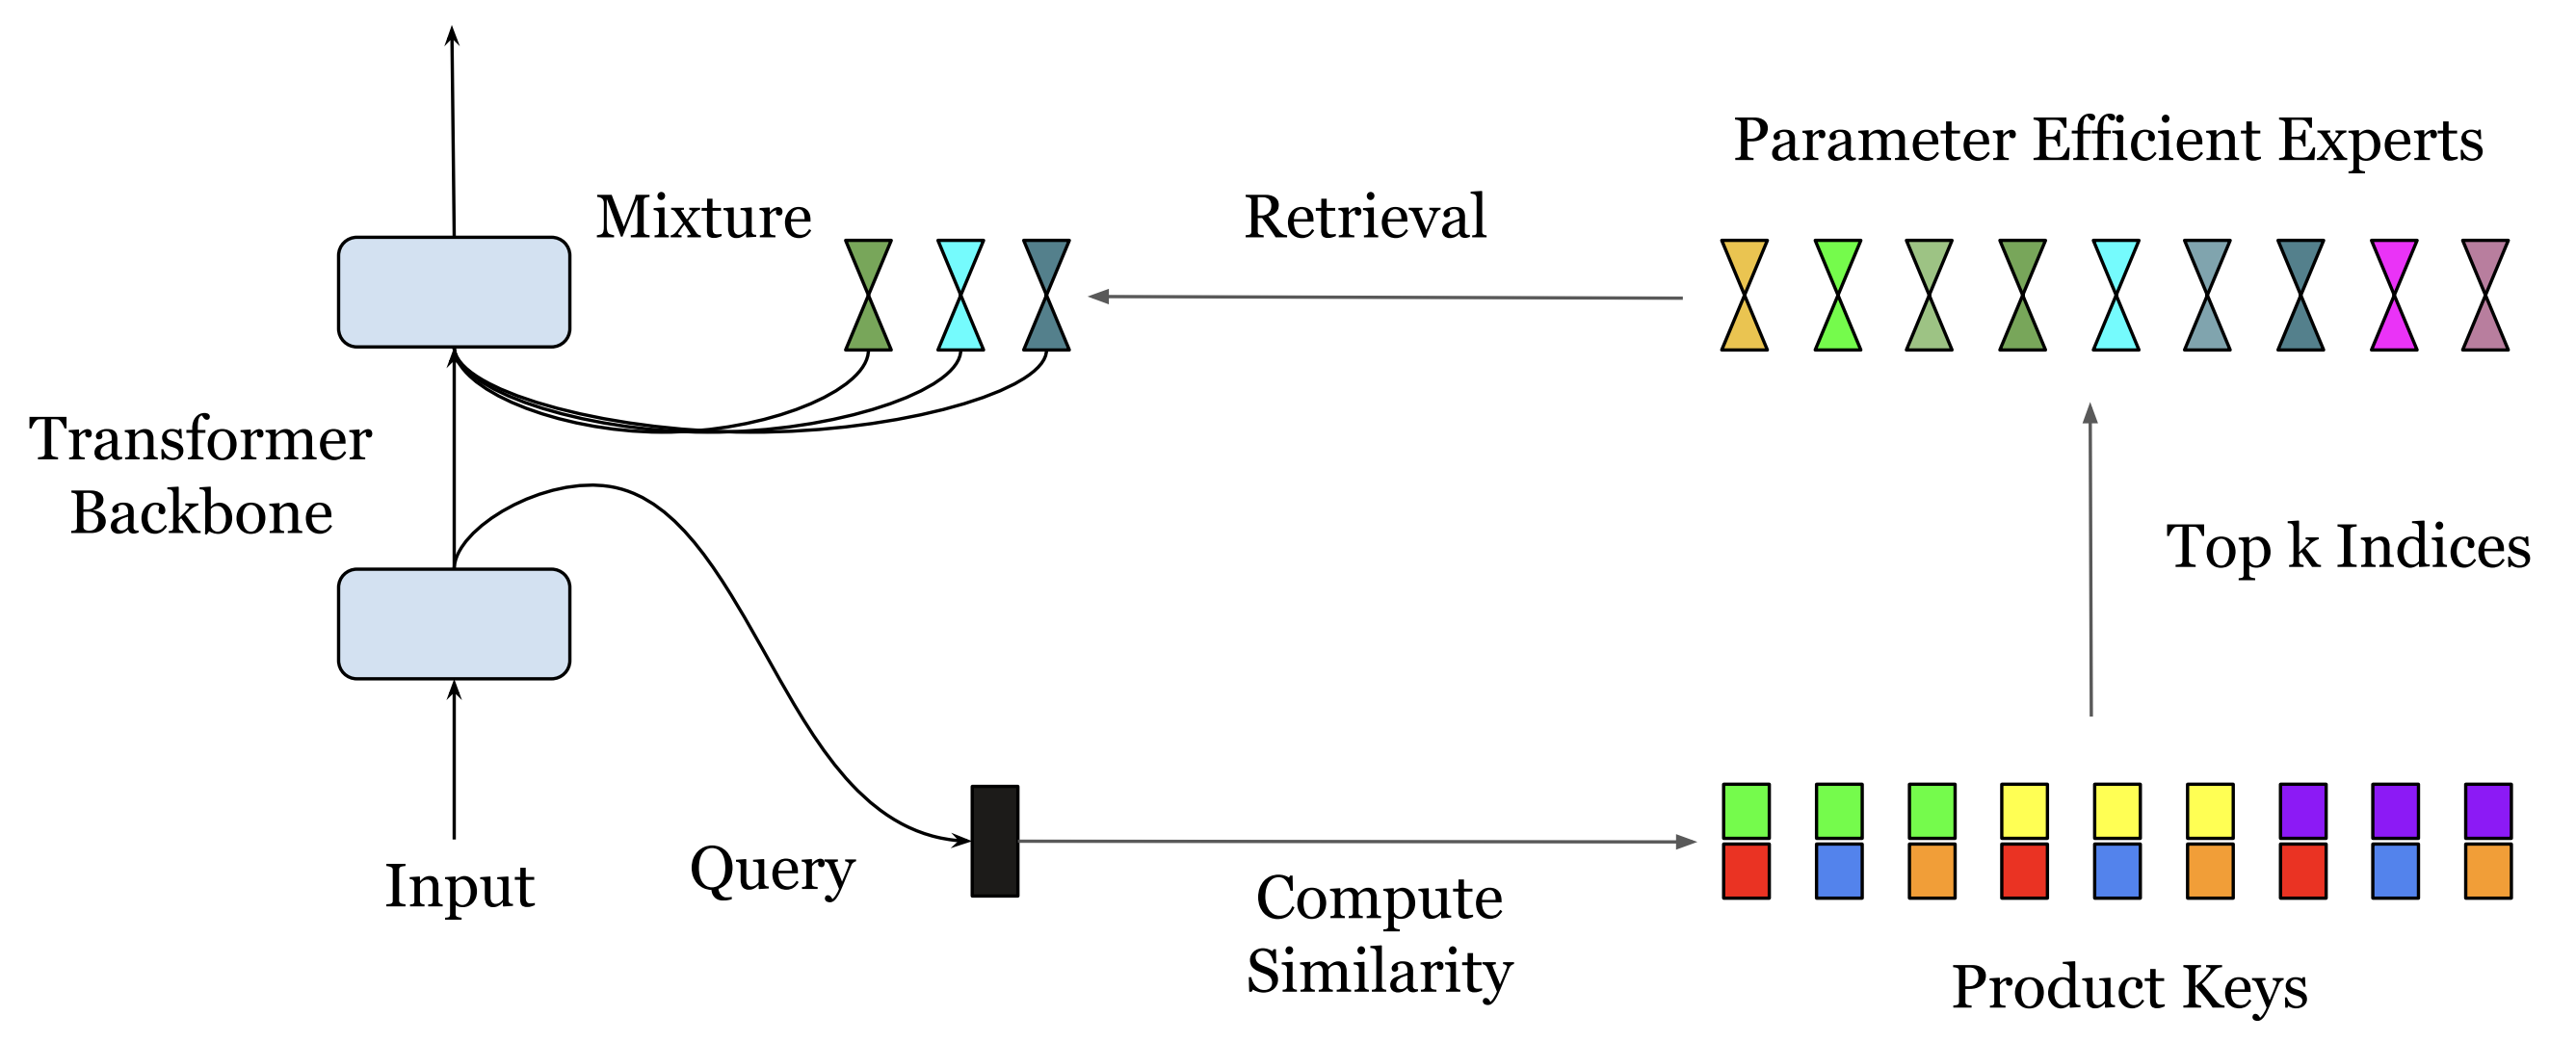
\includegraphics[width=1.0\linewidth]{figures/peer.jpg}
    \caption{PEER架构\cite{He2024MixtureOA}}
    \label{fig:PEER}
\end{figure}

具体来说，每个专家被实现为一个单神经元的多层感知机（MLP），其计算可以表示为：
\begin{equation}
    E_i(x) = \sigma(x\cdot u_i) v_i
\end{equation}
其中，$u_i$和$v_i$是专家的可学习参数（向量）。当一个输入$x$通过类似PKM的路由器检索到第$i$个专家时，模型取回的是参数$u_i$和$v_i$，并利用它们对$x$进行计算。这种设计使得每个专家的行为是输入依赖的（input-dependent），而不仅仅是返回一个固定的值，从而更贴近“专家”的本质。

PEER将专家粒度降至单个神经元，成功构建了一个拥有一百万个微型专家的混合专家模型，并在实验中证明了其在性能与计算成本权衡方面的优越性，为极大化专家数量的思路提供了有力支持。

\subsection{Ultra-Sparse Memory Network (UltraMem)}
Huang等人提出的Ultra-Sparse Memory Network (UltraMem)\cite{Huang2024UltraSparseMN} 旨在进一步解决PKM和PEER等架构在扩展到更大规模时遇到的性能和效率瓶颈。UltraMem通过引入更先进的组件和并行策略，显著提升了模型的表达能力和训练效率。其核心改进包括塔克分解查询密钥检索（Tucker Decomposed Query-Key Retrieval, TDQKR）、隐式值扩展（Implicit Value Expansion, IVE）以及一种高效的并行计算策略。

\subsubsection{塔克分解查询密钥检索 (TDQKR)}
TDQKR（图\ref{fig:tucker}）是对PKM中简单的加性评分机制的重大升级。PKM假设行、列子密钥的贡献是独立的（$s_{ij} = s_i + s_j$），这限制了路由的表达能力，并可能导致“拓扑偏差”（即Top-2密钥很可能与Top-1密钥在同一行或同一列）。TDQKR通过引入一个可学习的、低秩的“塔克核心”（Tucker core）张量$C \in \mathbb{R}^{r \times r}$来捕捉子密钥之间更复杂的乘性交互关系，其中$r$是塔克分解的秩。其得分矩阵的计算方式可以近似为：
\begin{equation}
    S_{\text{grid}} \approx \sigma_{\text{topM}}(S_{\text{row}}^T \times C \times S_{\text{col}})
\end{equation}
这里，$S_{\text{row}}$和$S_{\text{col}}$是查询与子密钥交互后得到的分数张量。这种设计允许模型学习到更灵活、更具表达力的路由模式，打破了简单的加性组合的局限，从而提高了专家选择的准确性。

\begin{figure}[h]
    \centering
    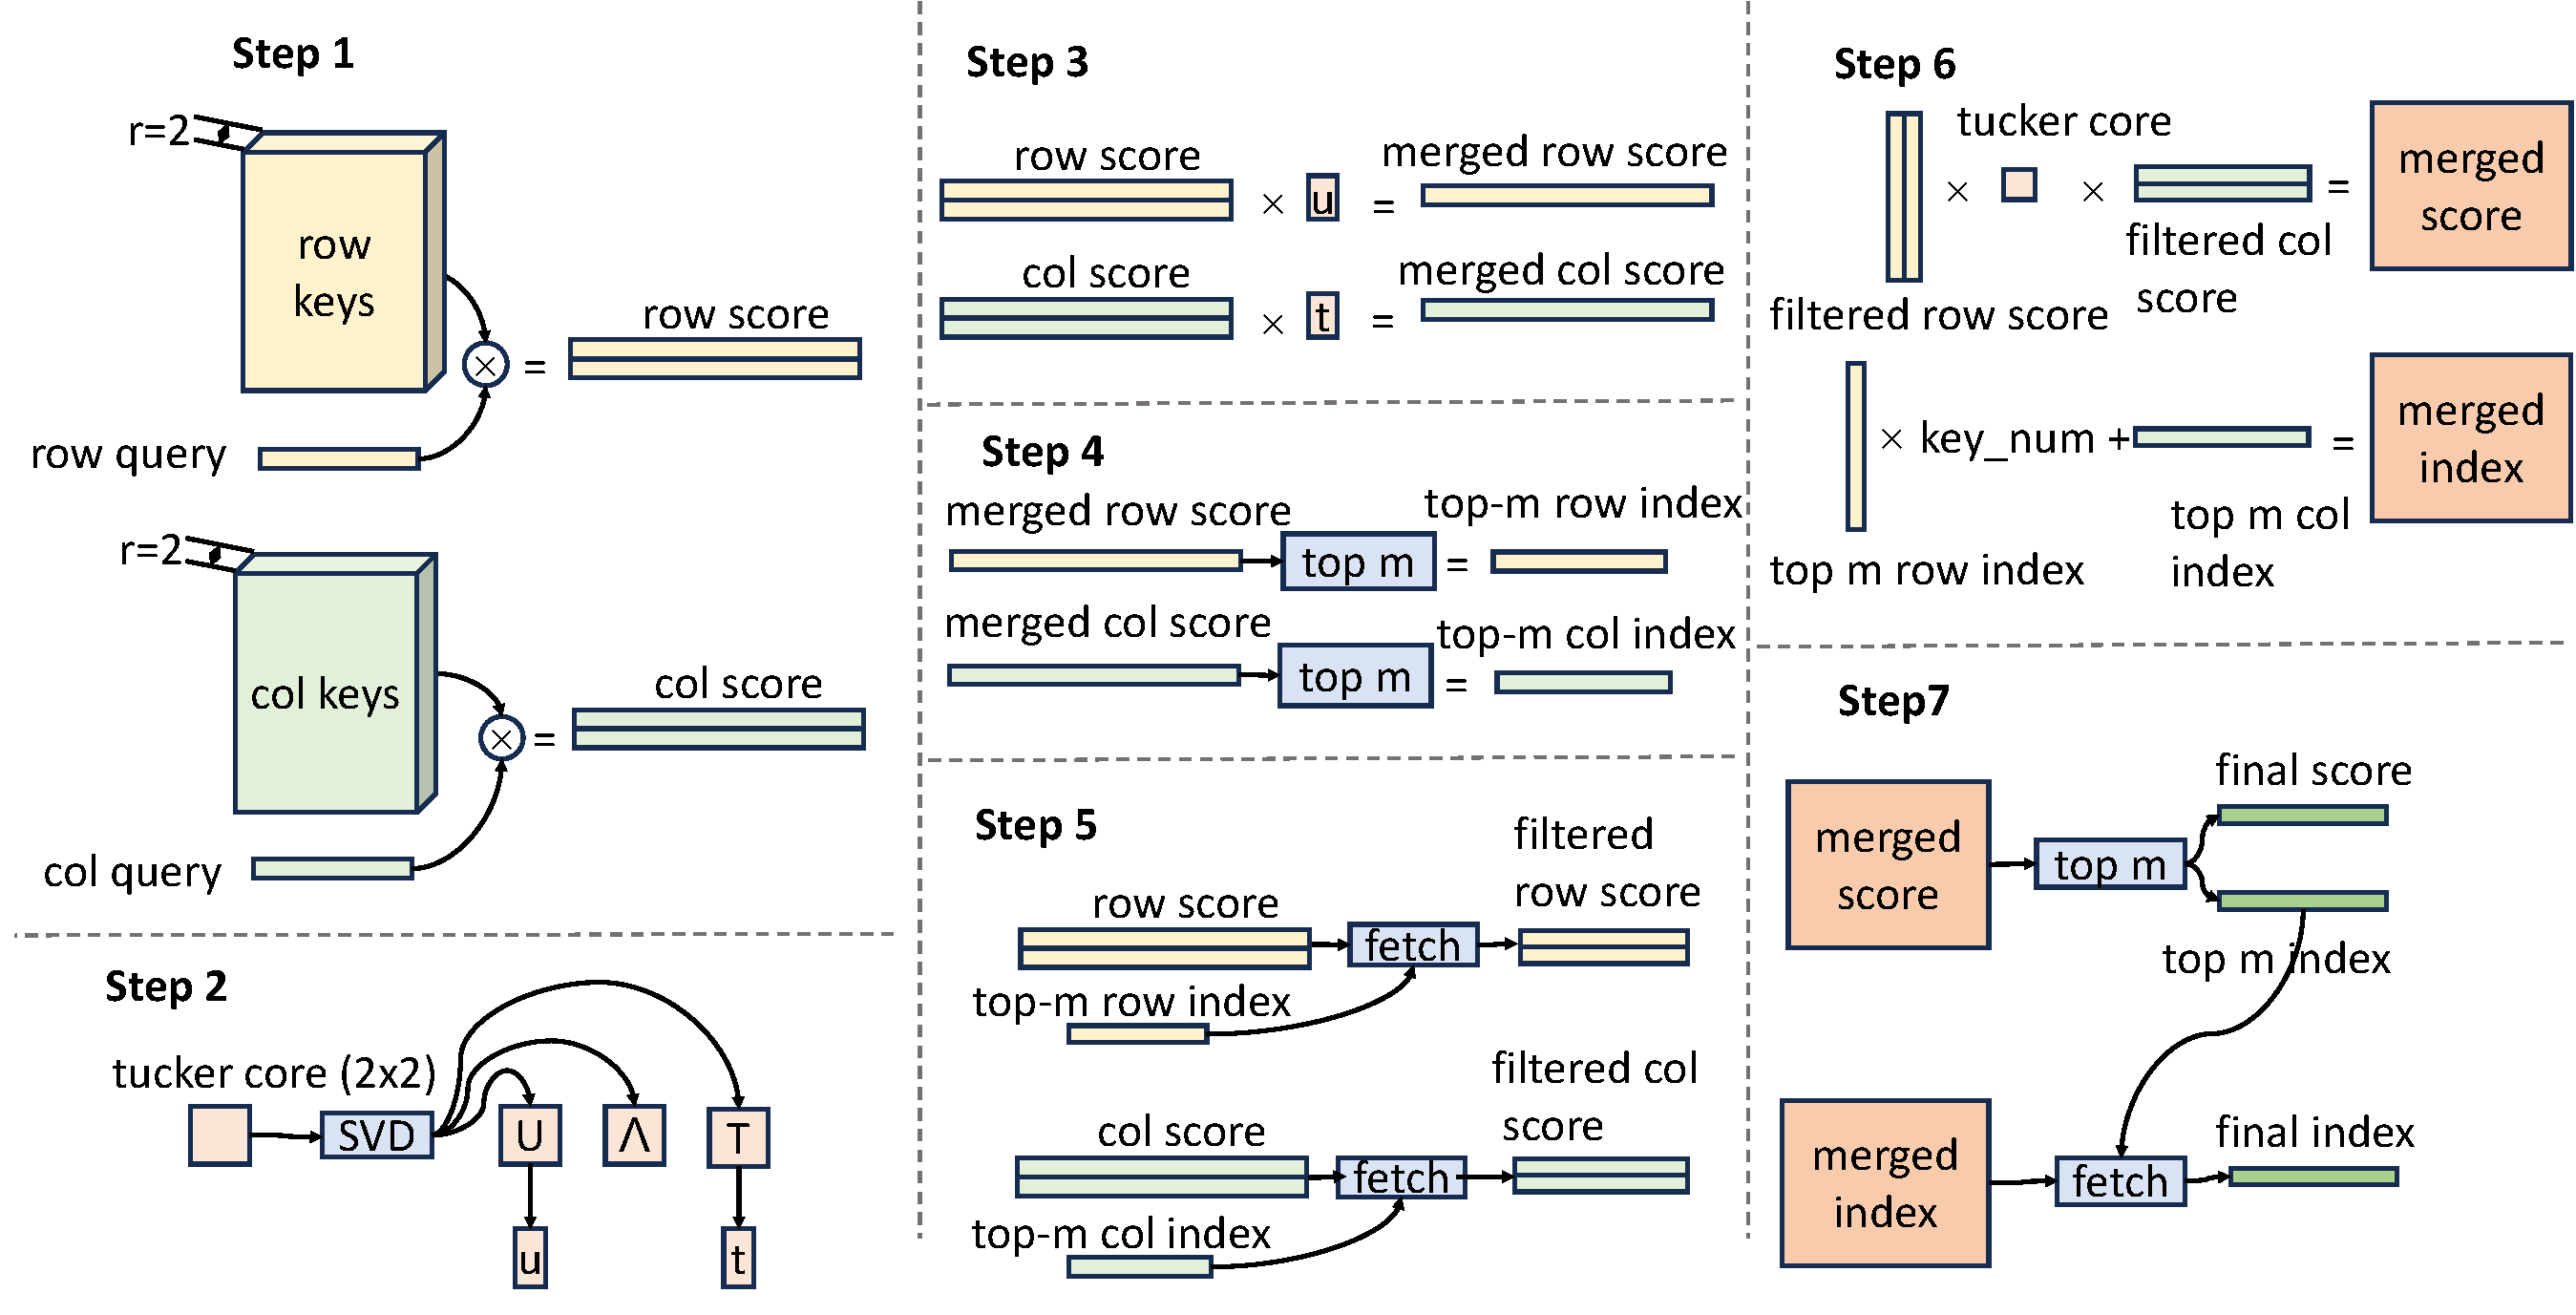
\includegraphics[width=1.0\linewidth]{figures/tucker_big.pdf}
    \caption{塔克分解查询密钥检索 (TDQKR)\cite{Huang2024UltraSparseMN}}
    \label{fig:tucker}
\end{figure}

\subsubsection{隐式值扩展 (IVE)}
IVE（图\ref{fig:ive}）是一种在不显著增加物理存储和访存开销的前提下，虚拟地扩大模型容量的技术。其动机是在保持计算效率的同时，进一步增加参数量。IVE将物理存储的值向量$V$（较小）通过一组$E$个可学习的线性投影矩阵$\{W_p\}_{p=1}^E$动态地生成多个“虚拟值块”$\tilde{V}_p = V W_p$。最终的输出是对这些虚拟值块的加权求和，计算可以被优化为“按需”进行：
\begin{equation}
o = \sum_{p=1}^E \tilde{V}_p^T \hat{s}_p = \sum_{p=1}^E W_p^T(V^T \hat{s}_p)
\end{equation}
其中$\hat{s}_p$是对应第$p$个虚拟块的得分。这种方式避免了在内存中实例化所有巨大的虚拟值参数，而是在计算时动态生成，从而以极小的额外计算代价实现了参数量的大幅扩展。

\begin{figure}[h]
    \centering
    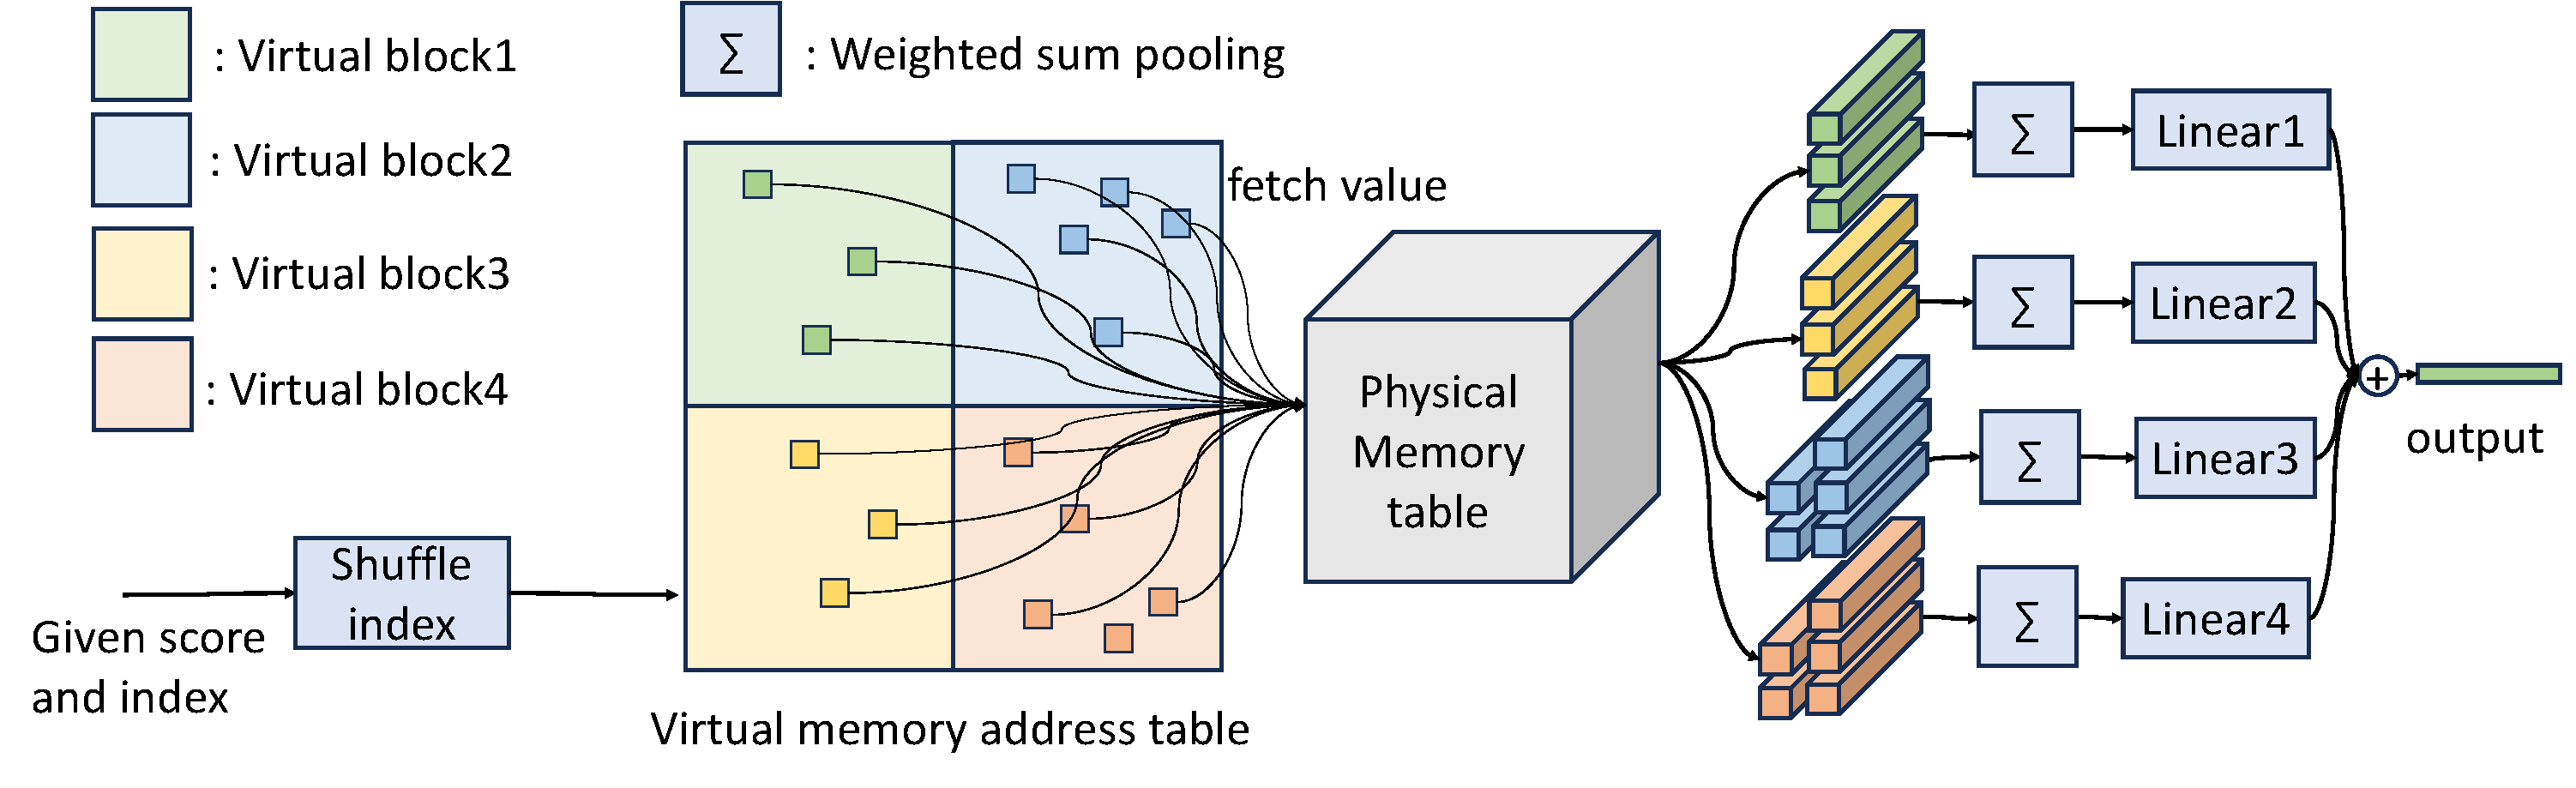
\includegraphics[width=1.0\linewidth]{figures/value_proj_big.pdf}
    \caption{隐式值扩展 (IVE)\cite{Huang2024UltraSparseMN}}
    \label{fig:ive}
\end{figure}

\subsubsection{并行计算策略}
为了提升训练效率，UltraMem采用了一种巧妙的并行策略。它并非将一个巨大的记忆层集中放置在模型某处，而是将多个较小的记忆层分散地插入到Transformer的不同块之间，形成一种“交错式”（interleaved）的架构（图\ref{fig:ultra_parallel}）。

\begin{figure}[h]
    \centering
    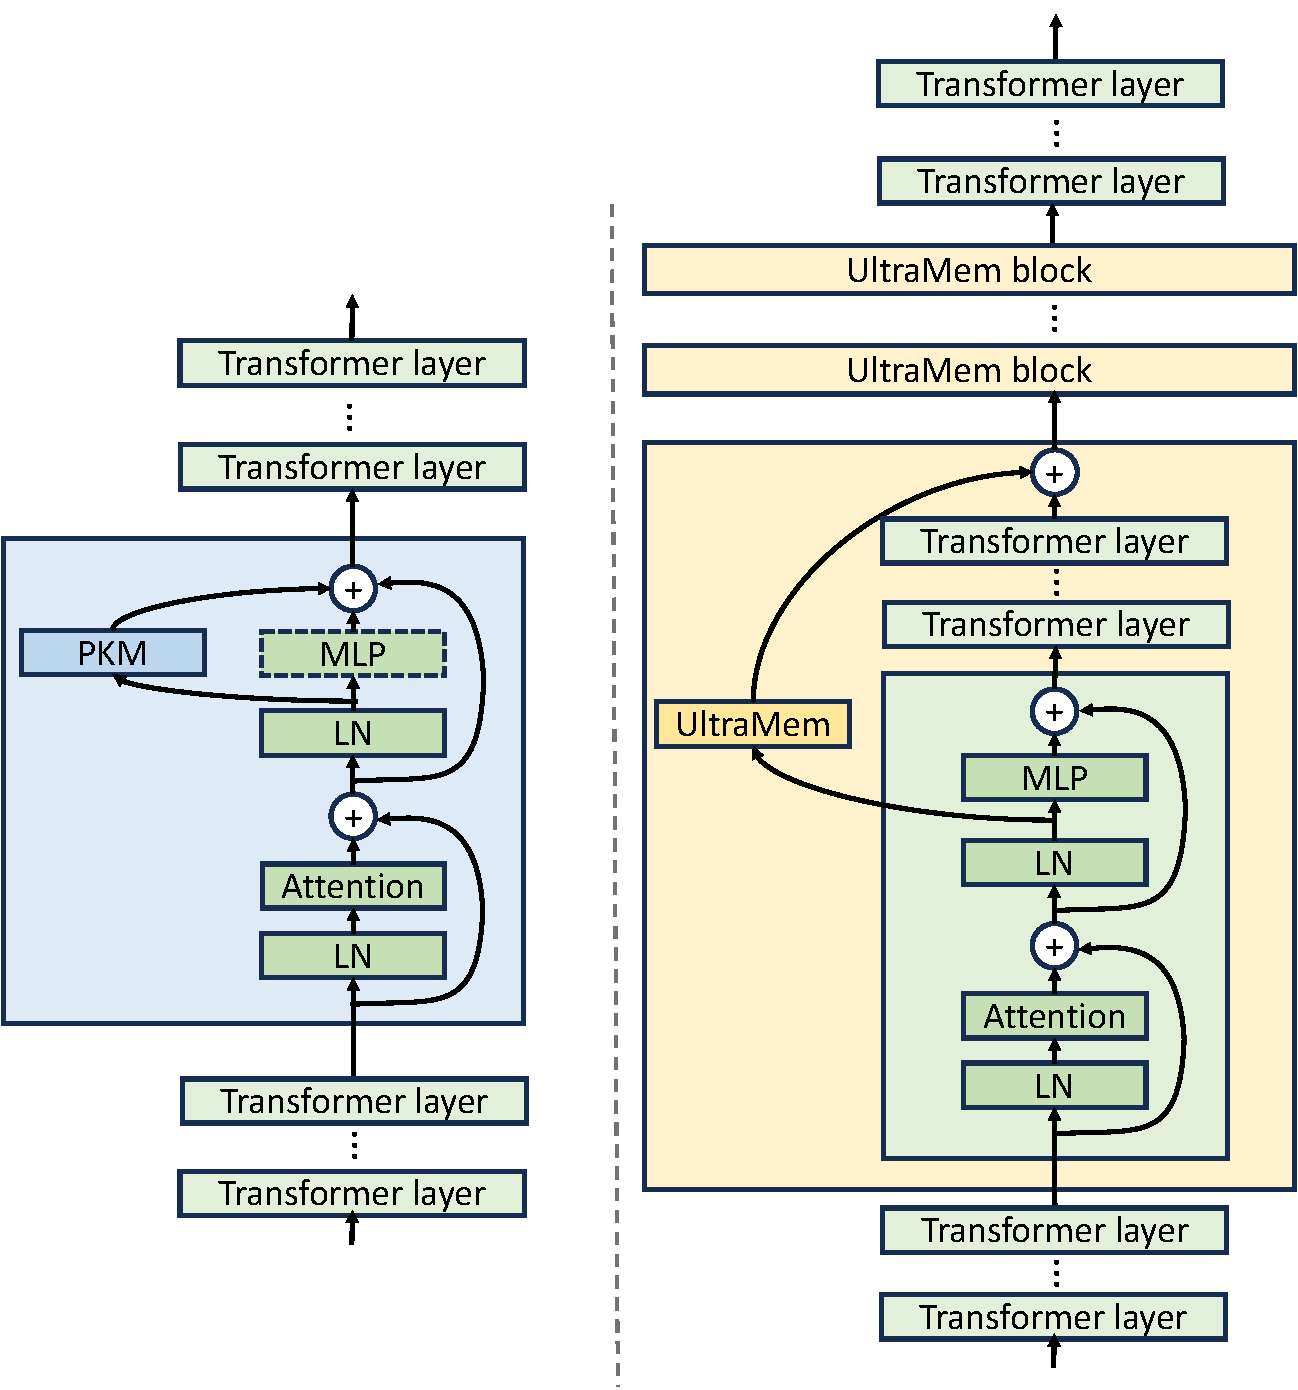
\includegraphics[width=0.7\linewidth]{figures/overall_structure.pdf}
    \caption{UltraMem的并行策略\cite{Huang2024UltraSparseMN}}
    \label{fig:ultra_parallel}
\end{figure}

这种策略的核心优势在于利用了不同类型计算层的硬件特性。标准的Transformer层（如自注意力和FFN）是“计算密集型”（compute-bound）的，其瓶颈在于处理器的浮点运算速度。而UltraMem的记忆层主要是“内存带宽密集型”（memory-bound）的，其瓶颈在于从GPU内存中读取大量密钥和值。

通过将这两种不同特性的层交错放置，可以实现\textbf{计算与访存的重叠（overlap）}。当GPU为一个Transformer块执行计算密集型操作时，数据预取机制可以异步地为下一个UltraMem层从内存中加载数据。反之，当GPU等待内存数据访问时，它可以处理其他计算任务。这种异步执行的流水线模式能够有效隐藏内存访问延迟，提升GPU的整体利用率，从而显著加快模型的训练速度。

\subsubsection{UltraMemV2}
在 UltraMem 的基础上，Huang 等人进一步提出了 UltraMemV2\cite{Huang2025UltraMemV2MN}（图\ref{fig:ultra_mem_v2}），其目标是使基于记忆的极细粒度专家架构在性能上能够与业界顶尖的、拥有 8 个激活专家的传统混合专家模型相媲美。为了实现这一目标，UltraMemV2 进行了一系列关键的架构和训练策略改进，成功地弥合了记忆层架构与主流稀疏模型之间的性能鸿沟。

\begin{figure}[h]
    \centering
    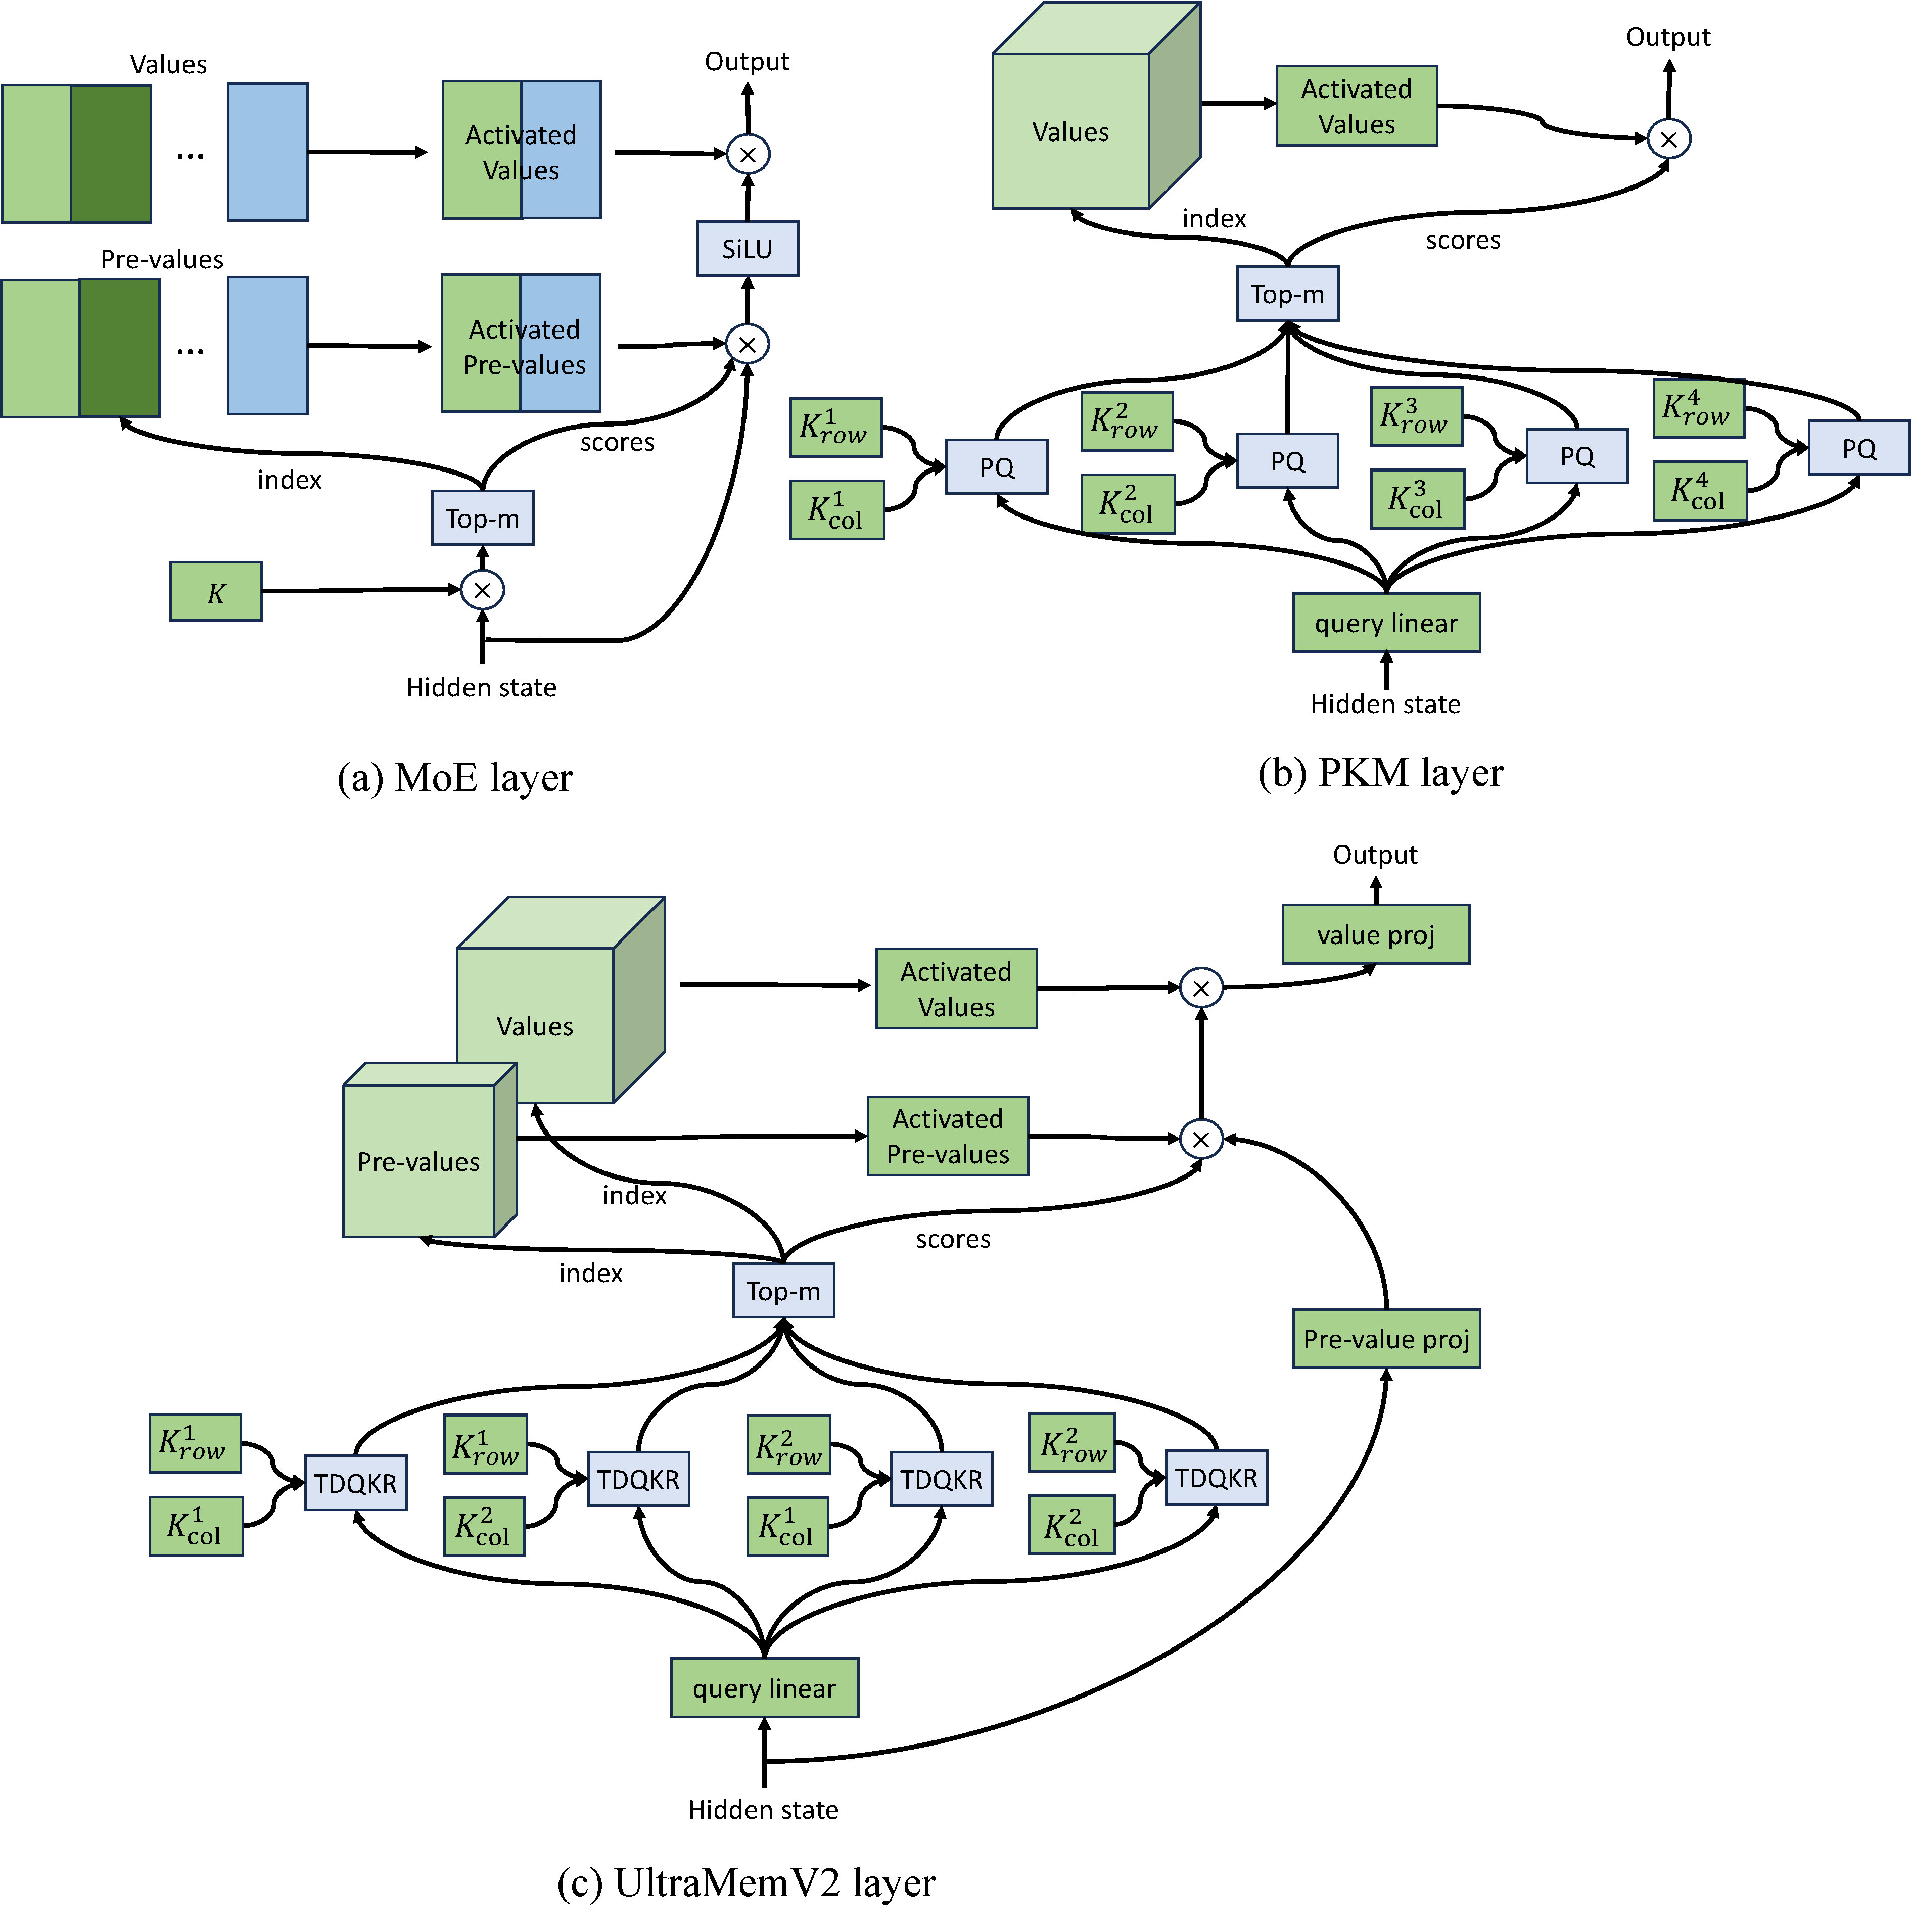
\includegraphics[width=1.0\linewidth]{figures/3structure.pdf}
    \caption{UltraMemV2和先前工作的对比\cite{Huang2025UltraMemV2MN}}
    \label{fig:ultra_mem_v2}
\end{figure}

UltraMemV2 的核心思想是通过五项关键改进来提升模型性能与效率：

\begin{enumerate}
    \item \textbf{架构集成（Architectural Integration）：} 将记忆层更紧密地集成到模型中。不同于以往模型仅在部分层插入记忆模块，UltraMemV2 在每一个 Transformer 块中都包含一个 UltraMemV2 层，使其与稠密计算部分深度融合，从而增加了稀疏参数的参与度。

    \item \textbf{简化的值扩展（Simplified Value Expansion）：} 对 UltraMem 中的隐式值扩展（IVE）机制进行简化。原始的 IVE 为每个虚拟内存块使用独立的线性投影层，这增加了非计算操作的开销。UltraMemV2 将其简化为使用单个共享的线性投影层来处理所有激活的值，如公式 \ref{eq:ultramemv2_ive} 所示。这一改动在保留模型容量的同时，显著提升了推理速度。
    \begin{equation}
        \boldsymbol{y} = \boldsymbol{W}_{\text{shared}} (\boldsymbol{V}^\top \hat{\boldsymbol{s}})
        \label{eq:ultramemv2_ive}
    \end{equation}
    其中 $\hat{\boldsymbol{s}}$ 是经过路由和排序后的得分向量，$\boldsymbol{V}$ 是物理值存储，$\boldsymbol{W}_{\text{shared}}$ 是所有虚拟块共享的单个线性投影。

    \item \textbf{类专家的值处理（Expert-like Value Processing）：} 借鉴 PEER 的思想，采用基于前馈网络的值处理方式。传统记忆网络检索的是静态的值向量，而 UltraMemV2 将其替换为动态的、依赖于输入的单神经元计算。具体而言，模型检索的不再是值向量本身，而是一个“预值”（pre-value）矩阵 $\boldsymbol{P}$。最终的输出通过一个前馈网络计算得出，如公式 \ref{eq:ultramemv2_peer} 所示。这种设计极大地增强了模型的表达能力。
    \begin{equation}
        \boldsymbol{y} = \boldsymbol{W}^\top (\boldsymbol{V}^\top \otimes ((\boldsymbol{P}\boldsymbol{x}) \otimes \hat{\boldsymbol{s}}))
        \label{eq:ultramemv2_peer}
    \end{equation}
    其中 $\boldsymbol{x}$ 是输入词元的表征，$\otimes$ 表示逐元素乘法。这一改动使得每个被激活的“专家”都能够根据当前输入动态地调整其输出。

    \item \textbf{优化的参数初始化（Optimized Initialization）：} 针对新架构设计了更符合理论的参数初始化方案。为了避免在训练大规模模型时可能出现的不稳定问题，UltraMemV2 的初始化策略确保了记忆层的输出激活方差与标准前馈网络层的方差保持一致，从而显著提升了训练的稳定性。

    \item \textbf{计算比例再平衡（Computational Rebalancing）：} 重新调整了记忆检索与前馈网络之间的计算量比例。通过实验分析，找到了一个最优的平衡点，以优化整体模型的性能。
\end{enumerate}

通过这些改进，UltraMemV2 成功地在各项基准测试中达到了与 8-expert 混合专家模型相当的性能，尤其在长上下文和记忆密集型任务上展现出优越性。这标志着极细粒度专家架构已发展成为一种兼具高效推理与强大性能的、有竞争力的稀疏模型方案。

% \subsection{专家选择的软性化 (Soft Expert Selection)}
% 与Top-k的“硬性”选择不同，一些研究探索了软性的路由机制，即每个词元与所有专家都进行交互，但交互的权重是稀疏的。这类方法虽然理论上更具表达力，但通常难以在现代硬件上实现高效计算，因此应用较少。
% FROM SPARSE TO SOFT MIXTURES OF EXPERTS
% Soft Merging of Experts with Adaptive Routing


% % MOA / MOM / MOR / MOD 
% [这里补充 MoH: Multi-Head Attention as Mixture-of-Head Attention]

% % topp; expert choice; Dynamic Mixture of Experts DYNMoE

% % 极细粒度的moe (PKM, peer / 字节的supermoe还是叫什么的)
% Large Memory Layers with Product Keys
% Mixture of A Million Experts
% ULTRA-SPARSE MEMORY NETWORK
% UltraMemV2: Memory Networks Scaling to 120B
% Parameters with Superior Long-Context Learning


% dense 2 sparse / sparse 2 dense之类的工作 https://arxiv.org/pdf/2410.08589
